\chapter{Implementación}

Una vez explicada la metodología, planificación y análisis, se va a proceder con explicación de la implementación de la solución. Así como en las otras secciones, se van a explicar todas y cada una de las decisiones tomadas, problemas encontrados y soluciones propuestas.

\section{Análisis de las posibles soluciones}

En este apartado, se analizarán las posibles soluciones para el desarrollo de la aplicación.

\subsection{Desarrollo de una \href{https://apps.nextcloud.com/}{aplicación} para \href{https://nextcloud.com/es/}{\textit{Nextcloud}}}

\textit{Nextcloud} es una plataforma de software libre que permite a los usuarios almacenar y sincronizar archivos, contactos, calendarios y más. Es una excelente opción para el desarrollo de nuestra aplicación, ya que proporciona una base sólida y una amplia gama de funcionalidades que pueden ser aprovechadas para implementar la funcionalidad de creación y gestión de memes. Para el desarrollo de una app en el ecosistema de \textit{Nextcloud}, se utiliza PHP y Vuejs. Además, \textit{Nextcloud} proporciona una API robusta que permite a los desarrolladores acceder a las funcionalidades del sistema.

Esta solución tiene varios problemas para el usuario o cliente final:

\begin{itemize}
    \item \textbf{Complejidad de la instalación:} La instalación de \textit{Nextcloud} puede ser complicada para los usuarios no técnicos. Por ejemplo para Ted Johnson González (experto conferenciante) que no tienen experiencia ni conocimientos técnicos podría ser un problema.
    \item \textbf{Consumo de recursos:} \textit{Nextcloud} es una aplicación bastante exigente en términos de recursos, especialmente si se gestiona una gran cantidad de datos o usuarios como podría ser el caso del departamento de marketing de Corporate Solutions. Desarrollando nuestra propia aplicación, podemos optimizar los recursos para que los requisitos sean mínimos.
\end{itemize}

Por otro lado, la implementación de base de funcionalidades como la sincronización en local y en remoto, el almacenamiento y la búsqueda de archivos y la gestión de usuarios no justifica el tiempo que se va a dedicar a adaptarse al \href{https://nextcloud.com/developer/}{entorno de desarrollo} que proporciona Nextcloud para desarrollar apps, ya que estas funcionalidades se pueden aplicar mediante la implementación de repositorios o desde cero con un coste de tiempo y recursos mucho menor.

\subsection{Desarrollo de una app móvil}

Otra posible solución sería el desarrollo de una aplicación móvil que permita a los usuarios crear y gestionar memes desde sus dispositivos móviles. Esta solución tiene varias ventajas, como la facilidad de uso y la accesibilidad, ya que los usuarios pueden elaborar memes en cualquier momento y lugar. Podría ser de bastante utilidad para todos y cada uno de los usuarios identificados.

Sin embargo, esta solución también tiene sus inconvenientes. Por ejemplo, el desarrollo de aplicaciones móviles limita bastante la audiencia a la que se puede llegar, puesto que no todos los usuarios tienen un dispositivo móvil o prefieren utilizar un ordenador. La idea de este proyecto es justamente el poder llegar a un público amplio y diverso, por lo que esta solución no sería la más adecuada.

\subsection{Desarrollo de una aplicación de escritorio}

En esta solución que se ha considerado es el desarrollo de una aplicación de escritorio que permita a los usuarios generar y gestionar memes desde sus ordenadores. Esta solución tiene varias ventajas como la facilidad que va a tener el usuario final para adaptarse a este tipo de entorno, pues es donde se realizan este tipo de tareas para que la edición pueda llegar a ser más compleja.

De nuevo, esta solución limita bastante la audiencia a la que se puede llegar, ya que no todos los usuarios tienen un ordenador o prefieren un dispositivo móvil (la cual es la mayoría actual).

\subsection{Desarrollo de una aplicación web}

El desarrollo de una aplicación web tiene lo bueno de las dos soluciones anteriores. Permite al usuario conectarse desde cualquier dispositivo sea PC o móvil. El desarrollo web es el más popular en la actualidad por lo que es bastante fácil encontrar comunidades, preguntas, documentación, artículos, etc.

La idea detrás de esta solución reside en una aplicación web que sea igualmente accesible desde cualquier dispositivo con conexión y un navegador adecuado. Una vez accedes a la plataforma web, puedes crear, editar, almacenar, compartir y buscar memes. La forma de almacenar los memes podría llegar a hacerse en local o en remoto.

\subsection{Conclusión}

El proyecto se va a desarrollar como una aplicación web teniendo esta usualmente una parte del cliente o frontend, una parte del servidor, api o backend y una parte de persistencia o base de datos. La elección de la tecnología en sendas partes es crucial a la hora de la experiencia de desarrollo, compatibilidad, escalabilidad, mantenimiento, etc.

\section{Milestones}

Como ya se ha explicado, el proyecto se dividirá en milestones o hitos. Cada uno de estos hitos representará un Producto Mínimo Viable (PMV), por lo que se irán generando entregables a lo largo de la implementación. En cada una de las siguientes subsecciones se describirá el producto que se generará en cada hito y las decisiones que se han tomado.

\section{Milestone 1: Modelo el problema}

El objetivo de este milestone es desarrollar un conjunto de definiciones de tipos en TypeScript para modelar los datos clave del dominio del problema, seguido de la implementación y prueba de dichas definiciones. Se crearán clases que representen los componentes principales del sistema, y se llevarán a cabo pruebas unitarias para verificar el correcto funcionamiento de las clases y sus métodos.

Para este desarrollo, se ha seguido un enfoque ágil combinado con Domain-Driven Design (DDD), lo que permite un modelado profundo del problema y un desarrollo incremental y continuo. Los requisitos se analizarán a través de historias de usuario, y se generará el código basado en DDD para estructurar los datos, garantizando una solución coherente y eficiente que se alinee con las mejores prácticas de desarrollo.

\subsection{Domain driven design}

Vamos a proceder al análisis del problema utilizando el diseño orientado al dominio (DDD), una metodología introducida por Eric Evans. Esta metodología de desarrollo de software nos ayudará a comprender y modelar el dominio empresarial, asegurando que nuestras soluciones se alineen con las necesidades específicas de los usuarios y del negocio.

DDD aborda la complejidad enfocándose en el `dominio' y promoviendo un `lenguaje ubicuo', un lenguaje común entre desarrolladores y partes interesadas para garantizar que el software refleje con precisión el ámbito empresarial. La modelización en DDD no busca crear el modelo más realista, sino uno útil y apropiado para su propósito~\cite{evans2004domain}.

El lenguaje ubicuo debe basarse en el modelo del dominio por lo que debe ser riguroso y preciso para evitar cualquier tipo de ambigüedad. De igual manera, debe ser especificado en una etapa temprana del proyecto por eso, está antes de todo el proceso. A continuación, algunos de los términos del lenguaje ubicuo:

\begin{itemize}
    \item \textbf{Meme}: imagen, vídeo o texto que difunde un mensaje que suele ser humorístico.
    \item \textbf{Plantilla}: formato base sobre la que se elaboran los memes.
    \item \textbf{Catálogo de memes}: almacenamiento centralizado de memes.
    \item \textbf{Colaborador}: usuario que puede editar un meme.
    \item \textbf{Visualizador}: usuario que puede ver un meme.
    \item \textbf{Búsqueda avanzada}: sistema de búsqueda en el catálogo de memes que permite filtrar memes por diferentes criterios.
\end{itemize}

Además de DDD, se han contemplado alternativas como el \textit{domain mapping} que facilita la visualización del dominio y \textit{volatility decomposisiton} que permite identificar las partes del sistema que son más propensas a cambios. Empresas como \textit{Netflix}, \textit{Uber} y \textit{Airbnb} han adoptado DDD con notable éxito como se detalla en esta~\href{https://blog.bitsrc.io demystifying-domain-driven-design-ddd-in-modern-software-architecture-b57e27c210f7}{publicación}.

Es importante destacar que DDD no abandona la filosofía ágil. Aunque esta metodología no está vinculada a otra metodología en particular, se orienta hacia la nueva familia de `procesos de desarrollo ágil'. Específicamente, asume que aplican dos prerrequisitos para aplicar el enfoque presentado en este libro: que el desarrollo sea iterativo y que la relación sea estrecha entre quiénes manejan el dominio y quiénes construyen el \textit{software}.

\subsubsection{Análisis de requisitos}

Los requisitos han sido identificados a partir de las historias de usuario~\ref{sec:historias_de_usuario} anteriormente definidas y los usuarios identificados en~\ref{sec:usuarios_identificados}. Estos requisitos son los que llamamos los requisitos básicos o esenciales a partir de los cuales se desarrollará el diseño.

\begin{itemize}
    \item \textbf{Se debe proporcionar un editor de memes.}
          \begin{itemize}
              \item[-] Historias de usuario requeridas: HU01, HU04 y HU02.
          \end{itemize}
    \item \textbf{Se debe proporcionar un catálogo de memes predefinidos.}
          \begin{itemize}
              \item[-] Historias de usuario requeridas: HU01, HU02 y HU03.
          \end{itemize}
    \item \textbf{La solución debe poder permitir colaboración en la creación de memes.}
          \begin{itemize}
              \item[-] Historias de usuario requeridas: HU04.
          \end{itemize}
    \item \textbf{Se debe proporcionar un sistema de búsqueda avanzada de memes.}
          \begin{itemize}
              \item[-] Historias de usuario requeridas: HU03.
          \end{itemize}
\end{itemize}

\subsection{Selección del lenguaje de programación}

Para la elaboración del código generado del DDD, se va a realizar un proceso de selección del lenguaje de programación en el que se va a escribir este código y posteriormente, realizar el proyecto.

\subsubsection{Criterios de búsqueda}

Los criterios que se han fijado para la búsqueda del lenguaje son los siguientes:

\begin{itemize}
    \item Compatible con el desarrollo web para su posterior utilización.
\end{itemize}

\subsubsection{Criterios de selección}

Las propuestas encontradas tras los criterios de búsqueda serán evaluadas según:

\begin{itemize}
    \item \textbf{Compatibilidad para desarrollo del cliente:} el lenguaje debe ser compatible con el desarrollo por la parte del cliente. Debe ser capaz de construir interfaces de usuario interactivas y dinámicas.
    \item \textbf{Ecosistema:} el lenguaje debe ser capaz de contar con numerosas alternativas a la hora de facilitar la programación. Esto incluye bibliotecas, frameworks, etc.
    \item \textbf{Sistema de tipos estáticos:} el lenguaje debe ofrecer este sistema de tipos estáticos que permita la detección temprana de errores, mejorando la seguridad, mantenibilidad, robustez, escalabilidad y documentación del código. Según~\cite{gao2017type} se concluyó que un lenguaje con tipificación estática como es TypeScript hubiera evitado el 15\% de los errores en el código de otro lenguaje sin tipificación como es JavaScript. Esto permite a los desarrolladores comprender mejor su código y detectar inconsistencias o errores mejora la capacidad de mantener y evolucionar el software con confianza y fiabilidad.
\end{itemize}

El desempeño de cada lenguaje en sendos criterios será etiquetado mediante la viñeta en el enumerado de los mismos desde \esp~si destaca por este criterio, \bien~si tiene un desempeño bueno sin llegar a destacar, \regular~si tiene un desempeño medio y \mal~si tiene un desempeño nulo.

\subsubsection{Propuestas}

\subsubsection{JavaScript}

\href{https://es.wikipedia.org/w/index.php?title=JavaScript&oldid=161023746}{JavaScript} es un lenguaje de programación de alto nivel, interpretado, orientado a objetos, basado en prototipos, imperativo y débilmente tipado y dinámico. Junto con HTML y CSS, JavaScript es una de las tres tecnologías fundamentales de la World Wide Web. Se utiliza principalmente del lado del cliente, implementado como parte de un navegador web. Todos los navegadores modernos interpretan código JavaScript. Fue desarrollado originalmente por Brendan Eich de Netscape con el nombre de Mocha, pasó por LiveScript y finalmente adoptó el nombre que tiene en la actualidad. Apareció por primera vez en el navegador Netscape Navigator en la versión 2002 en diciembre de 1995.

\begin{itemize}
    \item[\esp] \textbf{Compatibilidad para desarrollo del cliente:} compatible, fue originado exactamente para este propósito y como hemos mencionado. Se puede ejecutar directamente en la consola integrada en el navegador, es fácil de implementar aunque puede ser también un problema, ya que entre navegadores puede haber diferencias en la interpretación del código.
    \item[\esp] \textbf{Ecosistema:} tiene uno de los ecosistemas más grandes en el mundo de la programación incorporando todo tipo de bibliotecas y frameworks para facilitar el desarrollo. Algunos de los más conocidos son React, Angular, Vue, etc.
    \item[\mal] \textbf{Sistema de tipos estáticos:} es un lenguaje con tipado dinámico.
\end{itemize}

Por la parte del cliente es el lenguaje de programación más usado según la encuesta~\href{https://w3techs.com/technologies/overview/client_side_language}{W3Techs}.

\subsubsection{TypeScript}

\href{https://es.wikipedia.org/w/index.php?title=TypeScript&oldid=156203640}{\textit{TypeScript}}, un superconjunto de JavaScript desarrollado por Microsoft y publicado en octubre 2012, extiende JavaScript con una sintaxis basada en un sistema de tipos estático para ofrecer una detección temprana de errores y una integración más profunda con los editores de código.

Diseñado para compilarse a JavaScript, \textit{TypeScript} es compatible y válido con cualquier código JavaScript. Esta extensión facilita la escritura y el mantenimiento de aplicaciones a gran escala al proporcionar inferencia de tipos y herramientas avanzadas sin necesidad de código adicional. Con \textit{TypeScript}, los desarrolladores pueden definir tipos personalizados y recibir advertencias de errores directamente en el editor, lo que mejora significativamente la seguridad y eficiencia del proceso de desarrollo. A lo largo de los años, \textit{TypeScript} ha ganado popularidad por su capacidad para mejorar la calidad del código y facilitar el trabajo en proyectos complejos.

\begin{itemize}
    \item[\esp] \textbf{Compatibilidad para desarrollo del cliente:} es completamente compatible para el desarrollo del lado del cliente, incluso se puede ejecutar directamente en la consola integrada en el navegador.
    \item[\esp] \textbf{Ecosistema:} cuenta con uno bastante robusto y completo al igual que JavaScript. Incluye la mayoría de frameworks que se incluye JavaScript al ser completamente compatible con este.
    \item[\esp] \textbf{Sistema de tipos estáticos:} si por algo destaca TypeScript es por su sistema de tipos estáticos que permite detectar errores a la vez que se codifica mediante la comprobación de tipos evitando bugs, errores aportando seguridad, mantenibilidad y escalabilidad y seguridad al código. Además, incorpora características únicas como la inferencia de tipos, tipos genéricos, tipos de unión, tipos de intersección\ldots que lo vuelven mucho más flexible que otros lenguajes que también incorporan un sistema de tipos estático.
\end{itemize}

\subsubsection{Java}

\href{https://es.wikipedia.org/w/index.php?title=Java_(lenguaje_de_programaci%C3%B3n)&oldid=161108422}{Java} es un lenguaje de programación que fue desarrollado originalmente por James Gosling, de Sun Microsystems y posteriormente adquirida por su actual propietario, Oracle. La sintaxis deriva en gran medida de C/C++, pero cuenta con menos utilidades de bajo nivel. Las aplicaciones de Java son compiladas a bytecode que pueden ejecutarse en una máquina virtual Java sin importar la arquitectura de la computadora.

\begin{itemize}
    \item[\mal] \textbf{Compatibilidad para desarrollo del cliente:} no es compatible con el desarrollo por la parte del cliente, Java es más comúnmente utilizado en el lado del servidor y para desarrollar aplicaciones de escritorio.
    \item[\bien] \textbf{Ecosistema:} posee un ecosistema muy maduro con herramientas de desarrollo y frameworks como Spring para backend.
    \item[\esp] \textbf{Sistema de tipos estáticos:} tiene un sistema de tipos estáticos bastante estricto y el tipo de dato de un objeto no puede ser cambiado lo que aporta una robustez, fiabilidad y documentación al código bastante alto.
\end{itemize}

Por la parte del servidor, es el cuarto lenguaje de programación más usado según la encuesta~\href{https://w3techs.com/technologies/overview/programming_language}{W3Techs}.

\subsubsection{Python}

\href{https://es.wikipedia.org/w/index.php?title=Python&oldid=161467974}{Python} es un lenguaje de alto nivel de programación interpretado cuya filosofía hace hincapié en la legibilidad de código. Se trata de un lenguaje de programación multiparadigma que soporta parcialmente la orientación a objetos, programación imperativa y, en menor medida, programación funcional. Es un lenguaje interpretado, dinámico y multiplataforma. Python es uno de los lenguajes más populares en la actualidad. Fue desarrollado por Guido van Rossum en 1991.

\begin{itemize}
    \item[\mal] \textbf{Compatibilidad para desarrollo del cliente:} aunque compatible, no es el mejor lenguaje para dedicarlo al desarrollo por parte del cliente. Python es mucho más versátil y potente cuando se utiliza para el desarrollo por parte del servidor, en la ciencia de datos, inteligencia artificial, etc.
    \item[\bien] \textbf{Ecosistema:} tiene un ecosistema muy rico con una gran variedad de librerías y frameworks como puede ser \textit{Django} y \textit{Flask}.
    \item[\mal] \textbf{Sistema de tipos estáticos:} como hemos dicho anteriormente es un lenguaje con un sistema de tipos dinámicos.
\end{itemize}

\subsubsection{Ruby}

\href{https://es.wikipedia.org/w/index.php?title=Ruby&oldid=159723570}{Ruby} es un lenguaje de programación interpretado, reflexivo y orientado a objetos. El programador japonés Yukihiro Matsumoto, quien comenzó a trabajar en Ruby en 1993, lo presentó públicamente en 1995. Combina una sintaxis inspirada en Python y Perl con características de programación orientada a objetos similares a Smalltalk. Es interpretado de una sola pasada y su implementación oficial es distribuida bajo una licencia de software libre.

\begin{itemize}
    \item[\mal] \textbf{Compatibilidad para desarrollo del cliente:} es compatible, pero su verdadero potencial se encuentra por parte del servidor donde se desempeña de una manera excelente. Aun así, no es conocido por su rendimiento, sino por su facilidad a la hora de escribir código agilizando el desarrollo.
    \item[\bien] \textbf{Ecosistema:} \textit{Ruby on Rails}, Sinatra y Rack son algunos de los frameworks que utilizan Ruby. No es un ecosistema tan amplio como el de otros
    \item[\mal] \textbf{Sistema de tipos estáticos:} no es compatible, es un lenguaje dinámico.
\end{itemize}

Por la parte del servidor, es el tercer lenguaje de programación más usado según la encuesta~\href{https://w3techs.com/technologies/overview/programming_language}{W3Techs}.

\subsubsection{\MakeUppercase{Php}}

\href{https://es.wikipedia.org/w/index.php?title=PHP&oldid=161463562}{PHP} es un lenguaje de programación interpretado del lado del servidor y de uso general que se adapta especialmente al desarrollo web. Fue publicado inicialmente por Rasmus Lerdorf en 1994. El código de PHP suele ser procesado en un servidor web por un intérprete. En un servidor web el resultado de la interpretación y ejecución del código PHP sería HTML o una imagen binaria que formarían parte de la totalidad o parte de la respuesta.

\begin{itemize}
    \item[\mal] \textbf{Compatibilidad para desarrollo del cliente:} es compatible, pero es más conocido y es más un lenguaje interpretado por parte del servidor que por parte del cliente. El script php se puede incrustar directamente en el código html. Igualmente, este código se renderizaría en el servidor php y se enviaría al cliente.
    \item[\bien] \textbf{Ecosistema:} existen una gran variedad de herramientas como \textit{Laravel} y \textit{Symfony}. Estos frameworks son bastante usados en el backend.
    \item[\bien] \textbf{Sistema de tipos estáticos:} la calificación que más se ajustaría a su sistema de tipos sería: sistema de tipificación gradual (desde su versión 7.0 en adelante). Esta es una implementación que se sitúa entre un tipado estático y un tipado dinámico, es decir, algunas variables y expresiones pueden tener tipos y la corrección y tipificación se comprueba en tiempo de ejecución y otras en tiempo de compilación. Esto puede provocar inconsistencias en el código.
\end{itemize}

Por la parte del servidor, es el lenguaje de programación más empleado según la encuesta \href{https://w3techs.com/technologies/overview/programming_language}{W3Techs}.

\subsubsection{Go}

\href{https://es.wikipedia.org/w/index.php?title=Go_(lenguaje_de_programaci%C3%B3n)&oldid=158783243}{Go} es un lenguaje de programación concurrente y compilado con tipificación estática inspirado en la sintaxis de C pero con seguridad de memoria y recolección de basura. Ha sido desarrollado por Google y lanzado en 2009. También conocido como Golang, su objetivo era resolver los problemas de programación en un proyecto grande. Destaca por su minimalismo, simplicidad y eficiencia. Además, incorpora una sintaxis y estructura moderna y familiar. Algunos de los proyectos más conocidos que utilizan Go son Docker, Kubernetes, Terraform, etc.

\begin{itemize}
    \item[\mal] \textbf{Compatibilidad para desarrollo del cliente:} debido a su carácter compilado, no es compatible.
    \item[\regular] \textbf{Ecosistema:} no tiene un ecosistema muy amplio teniendo una comunidad no muy colaborativa y muy joven. Por lo general, si se quiere realizar algo en Go, tendrá que ser desde 0 y sin ningún framework. Esto más o menos se satisface con la simplicidad del lenguaje.
    \item[\bien] \textbf{Sistema de tipos estáticos:} incorpora un sistema de tipos estático lo que resulta de bastante ayuda a la hora de trabajar en proyectos grandes. Además, incorpora algunas características como la inferencia de tipos y tipos personalizados. Go es bastante criticado por no tener tipos genéricos.
\end{itemize}

\subsubsection{Kotlin}

\href{https://es.wikipedia.org/w/index.php?title=Kotlin_(lenguaje_de_programaci%C3%B3n)&oldid=160779037}{Python} es un lenguaje de programación multiplataforma, con tipificación estática, de alto nivel y de propósito general con inferencia de tipos. Fue desarrollado por JetBrains y lanzado en 2011 diseñado para ser totalmente interoperable con Java. En 2019 Google anunció que sería el lenguaje preferido para los desarrolladores de apps Android. Al igual que Java, es compilado a bytecode.

\begin{itemize}
    \item[\mal] \textbf{Compatibilidad para desarrollo del cliente:} Kotlin tiene soporte para la web compilando a JavaScript (backend Kotlin/JS) aunque su fuerte reside en el backend y en el desarrollo de aplicaciones móviles.
    \item[\regular] \textbf{Ecosistema:} la mayoría del desarrollo de librerías y frameworks se centra en el desarrollo de aplicaciones móviles y en el backend. Aun así, existe Kotlin Multiplatform que permite reducir el tiempo al escribir código compatible con diferentes plataformas manteniendo la flexibilidad y los beneficios de la programación nativa.
    \item[\bien] \textbf{Sistema de tipos estáticos:} como se ha mencionado anteriormente, implementa una tipificación estática con inferencia de tipos. Sin embargo, no se contempla la conversión implícita entre tipos.
\end{itemize}

\subsubsection{Scala}

\href{https://es.wikipedia.org/w/index.php?title=Scala_(lenguaje_de_programaci%C3%B3n)&oldid=161998724}{Scala} es un lenguaje de programación multi-paradigma diseñado para expresar patrones comunes de programación en forma concisa, elegante y con una tipificación fuerte y estática. La implementación actual se ejecuta en la máquina virtual de Java. Fue diseñado por Martin Odersky y lanzado en 2003.

\begin{itemize}
    \item[\mal] \textbf{Compatibilidad para desarrollo del cliente:} no es compatible y principalmente orientado a la parte del servidor y procesamiento de datos.
    \item[\mal] \textbf{Ecosistema:} tiene un ecosistema bastante centrado en campos como el procesamiento de datos y el backend. Sin embargo, Scala.js permite compilar a JavaScript.
    \item[\regular] \textbf{Sistema de tipos estáticos:} es un lenguaje con tipificación fuerte y estática aunque es bastante complejo y confuso. A todo esto se le añade que el compilador de Scala (sbt) es bastante lento y pesado.
\end{itemize}

\subsection{Conclusión}

Según los criterios de selección el lenguaje que más se adapta a los mismos sería TypeScript, ya que es compatible con el desarrollo del cliente, tiene un ecosistema amplio y un sistema de tipos estáticos con características particulares que lo hace único.

En comparación con su subconjunto, JavaScript, la diferencia principal no reside en la detección de errores en sí (que también) sino en qué se confía para detectarlos. Los programadores que escriben en JavaScript tienen que apoyarse en herramientas como los tests, linters para detectar errores de tipos mientras que TypeScript lo hace de forma ``nativa''. Si es verdad que el tipado supone un costo adicional al añadir un paso más, pero TypeScript en particular, reduce este coste usando tipos estructurales en vez de nominativos y haciendo inferencias.

En cuanto a su diferencia y lo que lo hace único respecto a este tipo de lenguajes con tipificación estática como Java, Kotlin, Go, Scala y PHP es su optimización del coste de la tipificación mediante la inferencia de tipos y sobre todo, por su tipificación estática basada en estructuras. Esto permite considerar estructuras como equivalentes cuando dos estructuras tienen diferente nombre y campos idénticos. Sin embargo, en los otros lenguajes con tipificación estática nominativa estas estructuras serían consideradas diferentes.

Por último, a modo de apunte, Go tiene una implementación híbrida entre tipificación basada en estructuras y nominativa, ya que puede llegar a verificar el tipo de los campos de la estructura.

\subsection{Gestor de paquetes}

Tras seleccionar el lenguaje de programación, se procedió a elegir un gestor de paquetes para la gestión de dependencias. En este proyecto, se ha optado por \textit{pnpm}, una herramienta que ha demostrado ser más rápida y eficiente que otras alternativas como \textit{npm} y \textit{yarn}. \textit{Pnpm} utiliza un algoritmo de enlaces simbólicos que permite almacenar una única copia de cada paquete en el disco, reduciendo significativamente el espacio utilizado y el tiempo de instalación, al mismo tiempo que mantiene compatibilidad con los gestores mencionados.

Aunque \textit{npm} ha sido el estándar tradicional, pnpm ha emergido como una alternativa sólida, ofreciendo mejoras notables en rendimiento y gestión de dependencias. Además, su comunidad activa y su mantenimiento regular garantizan su continuidad y evolución. Se destaca especialmente por su velocidad, siendo hasta un 60\% más rápido que sus competidores, según diversos \textit{benchmarks}, y por gestionar las dependencias de manera más segura, limitando el acceso de cada paquete únicamente a sus propias dependencias, lo que disminuye los riesgos de vulnerabilidad.

\subsection{Selección de la herramienta de testeo}

Antes de comenzar con el desarrollo, es necesario seleccionar la herramienta de testeo que se va a emplear para asegurar la calidad del código porque el código que no está probado, está roto. Además de asegurarse de que el código cumple con las historias de usuario e issues, la implementación de estos también debe funcionar; aquí es donde entran en juego los tests.

Hasta ahora se ha explicado el porqué hacer tests, pero ¿qué tipo de tests hay que hacer?, ¿cómo se hacen?, ¿qué tipo de tests existen? Cuantos más tests se hagan y más casos de uso se contemplen en ellos, más robusto, fiable, seguro y libre de fallos será el código. A continuación, se explicarán los diferentes tipos de tests que se pueden hacer:

\begin{itemize}
    \item \textbf{Tests unitarios:} se encargan de probar una unidad de código, es decir, una función, clase, método, etc. Estos tests se encargan de comprobar cada funcionalidad desde un punto de vista lógico o de bajo nivel. De hecho, hoy en día se habla mucho del \textit{code coverage} o cobertura de código que es la cantidad de flujos que se han probado en los tests, cuanto más alto sea, más confianza se podrá tener en el código.
    \item \textbf{Tests de integración:} el proyecto suele constar de trozos de código que se comunican entre ellos, los tests de integración se encargan de verificar que estos funcionen correctamente. Esto resulta cada vez más útil cuanto más grande sea el proyecto por lo que en nuestro caso y en principio, no es nuestro mayor problema.
    \item \textbf{Tests \textit{end to end}:} se encargan de probar la funcionalidad de la aplicación desde el punto de vista del usuario. Se suele automatizar una simulación de un posible usuario final que interactúa con el sistema.
\end{itemize}

\subsubsection{Criterios de búsqueda}

Los criterios que se han fijado para la búsqueda de la herramienta de testeo son los siguientes:

\begin{itemize}
    \item Compatible con TypeScript.
    \item Aserciones y tests unitarios.
    \item CLI para ejecutar los tests.
\end{itemize}

\subsubsection{Criterios de selección}

Las propuestas encontradas tras los criterios de búsqueda serán evaluadas según:

\begin{itemize}
    \item \textbf{Cobertura de pruebas:} las herramientas para tests pueden incluir la posibilidad de hacer tests en diferentes niveles de abstracción. Este nivel de abstracción será lo que determine la evaluación de este criterio. Algunos de los tests que se pueden escribir con estas herramientas o frameworks suelen ser: \textit{end to end} tests, tests de componentes y test de integración.
\end{itemize}

\subsubsection{Propuestas}

\subsubsection{\textit{Jest}}

\textit{Jest} es un framework de testing \textit{JavaScript} originado por \textit{Facebook}. Usualmente, se utiliza para los tests unitarios. Es compatible con \textit{TypeScript} a través del paquete \textit{ts-jest}. \textit{Jest} destaca por su facilidad de uso y rapidez. Además, incluye funcionalidades como partir desde una configuración nula o casi nula, las snapshots que captura el estado de un objeto y lo expone para que sirva de referencia para debugear, los tests se realizan de forma paralela para maximizar la eficiencia. Además, incorpora una buena compatibilidad con muchos de los lenguajes, \textit{frameworks} y librerías más usadas.

En cuanto a cobertura de pruebas, \textit{Jest} destaca en los test unitarios y en los tests de integración donde tiene una gran api como \textit{it} y \textit{expect}. Sin embargo, para los tests \textit{end to end} se necesita de \textit{Puppeteer} que es una librería de \textit{Node} que proporciona una API para controlar Chrome o Firefox a través del protocolo de \textit{DevTools} o \textit{WebDriver DiDi}.

\subsubsection{\textit{Vitest}}

\textit{Vitest} es un framework de testing orientado a los tests unitarios. Fue concebido para complementar \textit{Vite} que es una herramienta para ayudar a mantener y construir aplicaciones web \textit{JavaScript}. Debido a su creación por y para \textit{Vite}, si no se utiliza esta herramienta para el desarrollo, se requerirá un mayor esfuerzo a la hora de configurar y ejecutar los tests. \textit{Vitest} es mayoritariamente compatible con la api de \textit{Jest}. Al igual que \textit{Jest}, es bastante simple y rápido el construir tests debido a su amplio catálogo de funcionalidades para la api como los importes globales, primitivos SSR y existencia de numerosos plugins para el amplio ecosistema actualmente existente.

En cuanto a cobertura de pruebas, \textit{Vitest} destaca en los test unitarios, en los tests de integración y sobre todo en la velocidad y modernidad donde se destaca por encima de \textit{Jest} y otros \textit{frameworks} de testing. Sin embargo, al igual que en \textit{Jest}, se necesita de \textit{Puppeteer} para realizar los tests \textit{end to end}.

\subsubsection{Cypress}~\label{subsec:cypress}

\textit{Cypress} es una herramienta de automatización de tests para aplicaciones web. Es compatible de forma nativa con \textit{TypeScript} sin necesidad de instalar ningún paquete adicional. Es una aplicación de código abierto. \textit{Cypress} destaca por su facilidad de uso, rapidez y eficiencia. Además, incluye funcionalidades como la grabación de los tests, la posibilidad de correr tests en diferentes navegadores (no a la vez), la posibilidad de hacerlos para diferentes resoluciones, etc. Está orientado al testing frontend, pero también se pueden test unitarios y de integración.

En cuanto a cobertura de pruebas, \textit{Cypress} destaca en los test \textit{end to end} donde es uno de los mejores \textit{frameworks} para este tipo de tests, teniendo una integración completa debido a que se ejecutan directamente contra el navegador. Esto puede llegar a ser un problema, pues todos los tests que se ejecutan en el navegador y el código no es evaluado en \textit{Node}, por ejemplo, sino en el navegador.

\subsection{Conclusión}

Tras analizar todas las herramientas para el desarrollo de pruebas y teniendo en cuenta los criterios de selección, la herramienta que mejor se ajusta a los mismos es Cypress. Cypress proporciona una excelente cobertura de pruebas sin necesidad de instalar paquetes adicionales, es compatible con TypeScript de forma nativa y destaca por ejecutar las pruebas directamente en un entorno de navegador. Este aspecto es fundamental, ya que permite simular la interacción real de un usuario con la aplicación web en su entorno nativo.

Otra ventaja es su capacidad para grabar las pruebas o capturar pantallas en caso de fallos, lo que facilita la depuración. También permite la ejecución en paralelo para maximizar la eficiencia. Por último, usar una sola herramienta para todas las pruebas no solo simplifica el proceso, sino que lo agiliza considerablemente.

\subsection{Producto Mínimo Viable}

Como entregable de este milestone se han definido las siguientes interfaces:

\begin{itemize}
    \item \textbf{Catalogue}: Responde a la historia de usuario HU03 debido al requisito de poder acceder a memes relevantes y atractivos fácilmente accesibles.
    \item \textbf{Meme}: es la unidad básica de contenido de la aplicación. Responde básicamente a todas las historias de usuario.
\end{itemize}

Estas interfaces se han definido e implementado en TypeScript en módulos \href{https://stackoverflow.com/q/21247278?stw=2 }{\textit{«d.ts»}} que se utilizan para proporcionar definiciones de tipos para luego, poder consumirlo en el código. Estos módulos se desarrollan para, desde JavaScript, obtener los beneficios de la comprobación estática de tipos.

Además, se han realizado tests unitarios a partir de las implementaciones de las definiciones, con el fin de verificar que las interfaces definidas cumplen con lo especificado en los módulos \textit{«d.ts»}.

\section{Milestone 2: Persistencia de datos}

El producto mínimo viable (PMV) o entregable resultante tras este hito consiste será un sistema que permita la gestión eficiente de las entidades, garantizando su almacenamiento y recuperación, además de proporcionar las pruebas correspondientes que comprueben la correcta ejecución de dichas operaciones. Este hito marca el inicio de la implementación del proyecto, por lo que también incluirá la elección de la tecnología para el desarrollo de la solución propuesta.

\subsection{Selección de la tecnología}

Anteriormente, se hizo la selección del lenguaje de programación que se iba a emplear para desarrollar código para el DDD, el cual es TypeScript. Ahora, el siguiente paso es seleccionar la tecnología que va a ser empleada junto con TypeScript para desarrollar la solución.

Actualmente, cuando nos referimos a una tecnología web nos referimos a un conjunto de herramientas o framework que nos permiten desarrollar de forma más rápida y eficiente ayudándonos con ciertas características ya implementadas de base como la gestión de rutas, la gestión de estados, la gestión de peticiones, etc.

Una vez aclarado a qué nos referimos por tecnología, vamos a proceder al proceso en sí conforme se ha ido haciendo anteriormente, es decir, pasando primero por los criterios de búsqueda, selección, propuesta y finalmente, las conclusiones y justificación.

\subsubsection{Criterios de búsqueda}

Los criterios de búsqueda que se han fijado son:

\begin{itemize}
    \item \textbf{Typescript}: el lenguaje de programación que se va a usar es TypeScript, por lo que la tecnología seleccionada debe ser compatible con TypeScript.
    \item La tecnología debe ser compatible con \textbf{React}, una de las bibliotecas de JavaScript más populares en la actualidad para el desarrollo de interfaces de usuario, y que también es compatible con TypeScript. Su selección como criterio de búsqueda se basa en la escasa deuda técnica que presenta, su rapidez de uso y su estatus como un estándar, demostrado su aplicación en entornos reales. Además, cuenta con una amplia cantidad de recursos, bibliotecas adicionales y un mantenimiento continuo y estable.
\end{itemize}

\subsubsection{Criterios de selección}

Las propuestas encontradas tras los criterios de búsqueda serán evaluadas según:

\begin{itemize}
    \item Reactividad: la tecnología debe ser reactiva, es decir, debe ser capaz de reaccionar a los cambios de estado de la aplicación de forma eficiente.
\end{itemize}

\subsubsection{Propuestas}

\subsubsection{React}

\href{https://react.dev/}{\textit{React}} es una biblioteca de JavaScript de código abierto para construir interfaces de usuario o componentes de la interfaz de usuario, desarrollada por Facebook y lanzada en 2013. Es una de las bibliotecas más populares y ampliamente utilizadas en la actualidad. React está diseñada para ayudar a los desarrolladores a crear aplicaciones con datos dinámicos, siendo simple, declarativa y fácil de integrar. Se centra exclusivamente en la interfaz de usuario, actuando como la Vista en los patrones de diseño. Además, puede integrarse con extensiones basadas en React que gestionan las partes no relacionadas con la interfaz de usuario de una aplicación web.

\begin{itemize}
    \item[\bien] En cuanto a reactividad es una de las mejores opciones y más empleadas desde siempre. Fue una de las primeras tecnologías que introdujo la reactividad como característica principal a la hora del diseño de interfaces de usuario.
\end{itemize}

Lo único en lo que podríamos ver un inconveniente es en que no es un framework completo, sino una librería, por lo que se necesitará de otras librerías para completar la aplicación, de aquí pueden surgir varios problemas como dependencias no actualizadas, incompatibilidades, falta de optimización, se añade peso a la aplicación, etc. Además, cuando se trata de aplicaciones grandes, React puede ser un poco más complicado de manejar que otros. Esto mismo puede generar cierta deuda técnica en el futuro al tener que integrar herramientas que ayuden a la hora de gestionar el estado.

\subsubsection{\textit{Next.js}}

\href{https://nextjs.org/}{\textit{Next.js}} es un marco web de desarrollo frontend de React de código abierto desarrollado por Vercel y Guillermo Rauch en 2016 que permite a los desarrolladores la renderización del lado del servidor y la generación de sitios web estáticos. \textit{Next.js} es una de las mejores opciones para el desarrollo de aplicaciones web modernas. Es el framework más popular y ampliamente utilizados en la actualidad.

Una de las mejores características que posee \textit{Next.js} es su soporte para el SEO que es esencial si quieres que tu aplicación sea indexada por los motores de búsqueda. Tiene soporte SSR, pero no lo hace de forma predeterminada. Por último, tiene integradas las rutas dinámicas, la pre-generación de páginas (renderizado prefijado) y la exportación estática. Estas funcionalidades son muy importantes a la hora de la construcción de aplicaciones web. Los casos de éxito son numerosos como TikTok, Notion, ChatGPT, Spotify, etc.

\begin{itemize}
    \item[\bien] Cuando hablamos de reactividad en una aplicación web, \textit{Next.js} ofrece muchas mejoras en este sentido aportando numerosas opciones de renderizado y optimización aportando características y componentes que lo facilitan en gran medida. Algunos de estos ejemplos son el componente Image, el componente Link, etc.
\end{itemize}

La incorporación de esas características únicas y diferenciadoras de \textit{Next.js} puede ser un problema a la hora de la escalabilidad de la aplicación, ya que puede ser que no se necesiten todas las características que ofrece y que se añada peso y lentitud a la aplicación. Además, la curva de aprendizaje puede ser un poco más pronunciada que con otras tecnologías.

\subsubsection{Astro}

\href{https://astro.build/}{Astro} es un nuevo marco de desarrollo de aplicaciones web de código abierto que permite a los desarrolladores crear sitios web rápidos y eficientes. Fue desarrollado por Fred K. Schott y lanzado en 2022. Astro se centra en la creación de sitios web estáticos y dinámicos, proporcionando una estructura para el desarrollo de aplicaciones web modernas. Es conocido por su simplicidad y facilidad de uso.

Astro se ha convertido en una de las mejores opciones para el desarrollo de aplicaciones web modernas. Esta tecnología emergente ha ganado popularidad en los últimos años, principalmente porque, de forma predeterminada, no añade código JavaScript a menos que sea necesario. Otra de sus características más destacadas es su agnosticismo hacia la interfaz de usuario, lo que lo hace compatible con bibliotecas como React, Preact, Svelte, Vue, entre otras. Además, dado que el lenguaje de la interfaz de usuario es un superconjunto de HTML (la extensión Astro), la experiencia de desarrollo resulta familiar y accesible.

\begin{itemize}
    \item[\regular] En cuanto a la reactividad, Astro, al igual que \textit{Next.js}, ofrece muchas mejoras en este sentido aportando numerosas opciones de renderizado y optimización. Sin embargo, es una tecnología que se centra más en la elaboración de una aplicación web estática.
\end{itemize}

Como se ha mencionado, Astro se centra más en la elaboración de una aplicación web estática, por lo que puede ser que no se adapte del todo a las necesidades de la aplicación.

\subsubsection{Conclusión}

Tras valorar cada uno de los criterios de selección de las diferentes tecnologías, se ha llegado a la conclusión de que la que mejor se adapta a las necesidades del proyecto y que más va a facilitar el desarrollo de la solución es \textbf{\textit{Next.js}}. Este marco de desarrollo web ofrece numerosas características y funcionalidades que influirán de forma positiva a lo largo de todo el proyecto. A mayores, el hecho de ser un framework por encima de una librería como React, va a facilitar la implementación de casi cualquier característica.

\subsection{Tecnología}

En esta subsección se va a proceder a la explicación de la implementación de la persistencia de datos en el proyecto. Cuando hablamos de esto, nos referimos a la capacidad de que un sistema almacene y recupere las entidades definidas en el proyecto. Este proceso es esencial para asegurar la consistencia de la información.

La tecnología que se va a emplear para esta parte es \href{https://www.prisma.io/}{Prisma}, que es una herramienta de mapeo relacional de objetos u ORM moderna y de código abierto para Node.js y TypeScript. Proporciona un cliente de base de datos de tipado seguro haciendo que el acceso a la base de datos sea fácil, intuitivo y robusto.

Un ORM elige de manera sistemática y predictiva qué tablas crear y usar y que sentencias SQL generar a partir de la implementación en código orientado a objetos. Prisma mejora esta idea e implementa un ORM con un tipado seguro ya mencionado anteriormente, un modelado de datos declarativo llamado \textit{schema}, una API de cliente automáticamente generada y consistente, agnosticismo a la base de datos, manejo de migraciones cosa que puede llegar a ser muy útil a la hora de modificar el esquema de datos. Todas estas ventajas que provee Prisma hacen que la implementación de la persistencia sea más sencilla, segura y eficiente.

\subsubsection{Esquema de la base de datos}

Como se ha mencionado anteriormente, el esquema que se va a utilizar a partir del cliente de Prisma es un declarativo. A partir de él se puede generar un gráfico de relaciones entre las entidades que se van a almacenar en la base de datos.

\begin{figure}[H]
    \caption{Esquema modelo base de datos.}
    \centering
    \vspace*{0.5cm}
    \includegraphics[scale=0.2]{figuras/prisma-orm.png}
\end{figure}

Como se puede ver en la figura se han definido dos entidades que son \textit{Meme} y \textit{Catalogue}. La entidad \textit{Catalogue} tiene una relación de uno a muchos con la entidad \textit{Meme}. Esto significa que un catálogo puede tener muchos memes, pero un meme solo puede pertenecer a un catálogo.

La entidad de catálogo tiene el campo de identificador, del título, de la descripción, fecha de creación y fecha de actualización junto con los memes que pertenecen a ese catálogo. La entidad de meme tiene el campo de identificador, del título, de la descripción, de la imagen, de la fecha de creación y de la fecha de actualización junto con el catálogo al que pertenece.

\subsection{Consideraciones de diseño en la base de datos}

Para el diseño de la base de datos del proyecto `Memes para todos', se han aplicado principios que aseguran la integridad referencial y la calidad en el manejo de los datos, cumpliendo con criterios técnicos de calidad y buenas prácticas en bases de datos relacionales.

El desarrollo de la base de datos ha sido implementado utilizando Prisma ORM. Prisma facilita la definición de esquemas de base de datos y garantiza la consistencia y escalabilidad de los datos, permitiendo además un manejo intuitivo de las relaciones entre entidades y asegurando integridad referencial.

\subsubsection{Integridad referencial}

Se han establecido relaciones entre las tablas mediante el modelo de datos, que define claves foráneas y asegura que las referencias entre entidades sean válidas. En este caso, se ha establecido una relación uno a muchos entre las entidades \textit{Catalogue} y \textit{Meme}, donde un catálogo puede contener varios memes, pero un meme solo puede pertenecer a un catálogo usando la notación \texttt{@relation} en el esquema de Prisma. Esto asegura que cualquier registro en la tabla \textit{Meme} incluya una clave foránea que haga referencia a un catálogo válido, evitando que existan memes huérfanos o sin asociación correcta en la base de datos.

\subsubsection{Restricciones y validaciones}

Prisma permite definir restricciones directamente en el esquema del modelo tales como @id, @default o @updatedAt. Estas establecen que ese campo identifique de forma individual e inequívocamente a cada registro de un modelo, que tenga un valor por defecto en el caso de ser el identificador se ha establecido que se genera un identificador globalmente único y por último, que se actualice ese campo cada vez que se modifique.

\subsubsection{Mejores prácticas Prisma ORM y Next.js}

Para la implementación de la persistencia de datos en el proyecto se han seguido las \href{https://www.prisma.io/docs/orm/more/help-and-troubleshooting/help-articles/nextjs-prisma-client-dev-practices}{mejores prácticas} recogidas en la documentación de Prisma para Next.js.

La misma dice que se debe inicializar el cliente de Prisma en un archivo separado y exportarlo para que pueda ser importado en cualquier parte de la aplicación. Esto se hace para evitar la creación de múltiples instancias del cliente de Prisma, lo que puede provocar problemas de rendimiento y de memoria. Esto ocurre debido a que cuando se ejecuta el entorno de desarrollo la caché de Node.js se limpia.

\section{Milestone 3: Interacción con memes}

El producto mínimo viable (PMV) o entregable resultante tras este hito consiste en un sistema que permita la interacción con los memes, es decir, un editor de memes que permita la creación y edición, por ahora, de los mismos.

El desarrollo del editor de memes es una parte fundamental del proyecto, ya que es una de las partes principales de cara al usuario final. El código ha sido desarrollado pensando en un canvas que es dónde se realiza la edición en sí. Alrededor del mismo se ubican las diferentes herramientas, funcionalidades y operaciones disponibles.

Este hito también se incluye la creación y ejecución de los tests correspondientes para comprobar las operaciones. Antes de comenzar con la explicación de la implementación se da paso a las diferentes decisiones técnicas que se han tomado.

En primer lugar, hay que decidir cómo implementar la parte del canvas. El implementar un motor de renderizado desde cero es una tarea que para nuestro caso, es impracticable debido a la cantidad de tiempo y recursos que se necesitarían. Por ello, se ha decidido emplear un motor de renderizado ya existente.

\subsection{Selección del motor de renderizado}

Como se ha mencionado anteriormente, se ha decidido usar un motor de renderizado ya existente como librería e incluirlo en el proyecto de forma que se va a proceder con la selección del motor.

\subsubsection{Criterios de búsqueda}

Los criterios de búsqueda establecidos para la selección de la biblioteca para el renderizado del canvas son:

\begin{itemize}
    \item \textbf{Compatibilidad con tecnologías ya seleccionadas}: la biblioteca seleccionada debe ser compatible con React y Next.js.
    \item \textbf{Con tipos}: la biblioteca debe estar escrita en TypeScript o tener definiciones de tipos.
\end{itemize}

\subsubsection{Criterios de selección}

Las propuestas serán evaluadas según los siguientes criterios:

\begin{itemize}
    \item \textbf{Integración}: debe ser fácil de integrar en el proyecto.
    \item \textbf{Mantenibilidad}: debe estar activamente mantenida y actualizada.
    \item \textbf{Rendimiento}: debe poder manejar gráficos incluso en condiciones de bajos recursos.
\end{itemize}

El desempeño de cada lenguaje en sendos criterios será etiquetado mediante la viñeta en el enumerado de los mismos desde \esp~si destaca por este criterio, \bien~si tiene un desempeño bueno sin llegar a destacar, \regular~si tiene un desempeño medio y \mal~si tiene un desempeño nulo.

\subsubsection{Propuestas}

\subsubsection{Konva.js}

Konva.js es una biblioteca o framework de código abierto que permite la creación de gráficos interactivos en el canvas para aplicaciones de escritorio y móviles. Permite animaciones, manejo de eventos, manipulación y anidación de nodos, capas y filtros. Este proyecto se tuvo sus inicios a partir de KineticJS (otra biblioteca del mismo estilo, pero que fue discontinuada, en 2014 fue su última actualización).

\begin{itemize}
    \item[\regular] \textbf{Integración:} Ha estado a punto de no entrar siquiera en la lista de propuestas, ya que necesita de una dependencia extra para funcionar en React (react-konva).
    \item[\bien] \textbf{Mantenibilidad:} Está activamente mantenida y actualizada. La última actualización el 9 del pasado mes. Sin embargo, la dependencia de react-konva no está tan actualizada siendo la última en 2019.
    \item[\bien] \textbf{Rendimiento:} Se ha demostrado que su rendimiento es bueno incluso en condiciones de bajos recursos.
\end{itemize}

Konva.js destaca por su alto rendimiento a la hora de manejar eventos y gestos, como el arrastre y el zum que los hace de manera muy eficiente. Sin embargo, el enfoque de capas y nodos puede resultar en una curva de aprendizaje bastante más pronunciada.

\subsubsection{Fabric.js}

\href{http://fabricjs.com/}{Fabric.js} es una biblioteca JavaScript de código abierto centrada en la manipulación de gráficos y objetos dentro del canvas. Permite la creación de gráficos interactivos, la manipulación de imágenes y la edición de texto.

\begin{itemize}
    \item[\esp] \textbf{Integración:} Gracias a su enfoque modular y orientado a objetos se integra fácilmente con las tecnologías seleccionadas anteriormente. No necesita ninguna dependencia extra para funcionar junto con React y tener el tipado de TypeScript.
    \item[\bien] \textbf{Mantenibilidad:} Se actualiza continuamente, siendo la última hace dos semanas.
    \item[\bien] \textbf{Rendimiento:} En cuanto a rendimiento es un framework bastante bueno no llegando a destacar.
\end{itemize}

Fabric.js destaca por su enfoque orientado a objetos lo que vuelve mucho más intuitivo la experiencia de desarrollo. Permite manejar elementos del canvas como objetos manipulables y editables. La desventaja que provee esta biblioteca puede residir en el rendimiento que no destaca tanto como otras bibliotecas.

\subsubsection{PixiJS}

PixiJS es un sistema de código abierto basado en la web que provee de un motor de renderizado de canvas potente para juegos, visualización de datos y otras aplicaciones que requieran de gráficos avanzados e intensivos.

\begin{itemize}
    \item[\regular] \textbf{Integración:} PixiJS necesita de una dependencia extra para poder llegar a un funcionar de manera óptima en React (pixijs-react).
    \item[\bien] \textbf{Mantenibilidad:} Está activamente mantenida y actualizada. La última actualización fue en marzo.
    \item[\esp] \textbf{Rendimiento:} PixiJS principalmente destaca por su rendimiento.
\end{itemize}

PixiJS está diseñada principalmente para el desarrollo de videojuegos de ahí, su rendimiento basado en la aceleración por hardware. Esto puede llegar a tener una desventaja y es, por ejemplo, en nuestro caso, que queremos algo más sencillo que no requiera de tanto rendimiento y que puede llegar a ser ejecutado en dispositivos de bajo rendimiento.

\subsubsection{Conclusión}

Después de evaluar las diferentes propuestas bajo los criterios establecidos, Fabric.js se destaca como la mejor opción para el proyecto de editor de memes online. Su enfoque orientado a objetos, facilidad de integración con React y TypeScript, junto con la asidua actualización y mantenimiento de la biblioteca, la convierten en la elección más adecuada para el desarrollo de la solución propuesta.

PixiJS, aunque, ofrece el mejor rendimiento de entre las propuestas gracias a su aceleración por hardware, el enfoque hacia el desarrollo de videojuegos introduce una complejidad innecesaria para algo mucho más simplista. Konva.js, por su parte, presenta algunas limitaciones en cuanto a su integración con TypeScript y su ecosistema más pequeño. Aunque Konva.js tenga más descargas en npm que Fabric.js, la biblioteca de Fabric.js tiene una comunidad mucho más grande en GitHub~\href{https://stackshare.io/stackups/bower-pixi-js-vs-fabricjs-vs-konva#description}{según sus estrellas}.

En definitiva, Fabric.js no solo cumple con los requisitos de rendimiento y compatibilidad, sino que también ofrece una excelente mantenibilidad y soporte comunitario, asegurando que el proyecto pueda evolucionar de manera sostenible y con una deuda técnica mínima.

\subsection{Diseño de interfaces}

Antes de empezar a hablar de la implementación del editor en sí, se va a proceder a la explicación de la decisión tomada acerca del diseño de interfaces, ya que se ha tomado en este milestone al ser necesario implementar la interfaz.

El diseño de interfaces por lo general, conlleva consigo una elección de framework de UI y un catálogo o catálogos de componentes que ayuden, agilicen y provean de consistencia a la UI.

En nuestro caso todas las interfaces del proyecto se han implementado utilizando \textbf{\textit{Tailwind}} como framework de UI CSS y \textbf{\textit{ShadCN}}, un catálogo de componentes.

\subsubsection{Tailwind CSS}

Tailwind es un framework de CSS que se ha integrado en el desarrollo de estilos para componentes mediante el uso de clases directamente en el marcado. Es una herramienta ampliamente adoptada por aproximadamente el 50\% de los desarrolladores según la encuesta \href{https://2023.stateofcss.com/es-ES/css-frameworks/}{\textit{stateofcss}}. Su popularidad se debe, en gran medida, a su facilidad en la implementación, ya que permite definir estilos directamente en el lenguaje de marcado, simplificando el proceso de diseño.

Además, Tailwind se adapta perfectamente a Next.js, pues al crear un nuevo proyecto con Next.js, se ofrece la opción de incluirlo automáticamente en las dependencias sin ningún tipo de configuración extra, lo que refuerza su presencia como una solución casi nativa para los desarrolladores de esta plataforma.

\subsubsection{ShadCN}~\label{subsec:shadcn}

ShadCN es un conjunto de componentes UI que funciona como un catálogo para desarrollar interfaces de usuario, proporcionando una solución sólida, intuitiva, consistente y escalable para proyectos. Este catálogo está diseñado con un enfoque muy alineado con el ecosistema de Next.js, ya que incluye los mismos componentes que se utilizan en la página web oficial de Next.js y Vercel, la compañía que desarrolla y mantiene Next.js. Gracias a esta estrecha relación, ShadCN se convierte en una opción ideal para quienes ya tienen experiencia sobre Next.js en sus proyectos porque permite construir interfaces de usuario con la misma coherencia y calidad visual que la propia plataforma oficial de Vercel.

ShadCN ofrece una serie de componentes listos hechos a partir de Tailwind CSS que se pueden incluir en cualquier proyecto de React. Además, se puede personalizar fácilmente para adaptarse a las necesidades de la aplicación como colores, tamaños, etc. Además, están preparados para seguir con los estándares de las mejores prácticas de accesibilidad asegurando que la página sea accesible.

\subsubsection{Decisiones de diseño y prácticas}

Durante todo el diseño del proyecto se van a seguir una serie de buenas prácticas en cuanto al diseño. Estas prácticas van a tener de base a Tailwind y ShadCN. Algunas son:

\begin{itemize}
    \item \textbf{Adaptabilidad}: las interfaces implementadas van a ser diseñadas de base para que se adapten a cualquier dispositivo.
    \item \textbf{Consistencia visual}: una paleta de colores y tipografía coherente en todo el proyecto.
    \item \textbf{Experiencia de usuario}: para mejorarla se van a incorporar mejoras de calidad de vida, interactividad, animaciones, etc.
\end{itemize}

\subsection{Editor de memes}

El editor de memes se ha diseñado basado en una arquitectura modular, aprovechando las ventajas de React para gestionar el estado y la reactividad, en Fabric.js como motor para el renderizado y manejo de eventos del canvas y en \href{https://hammerjs.github.io/}{Hammer.js} para apoyar la cobertura de gestos táctiles (en nuestro caso tanto para el pellizco como para el desplazamiento).

\begin{figure}[H]
    \caption{Tema claro de la interfaz de usuario del editor.}
    \centering
    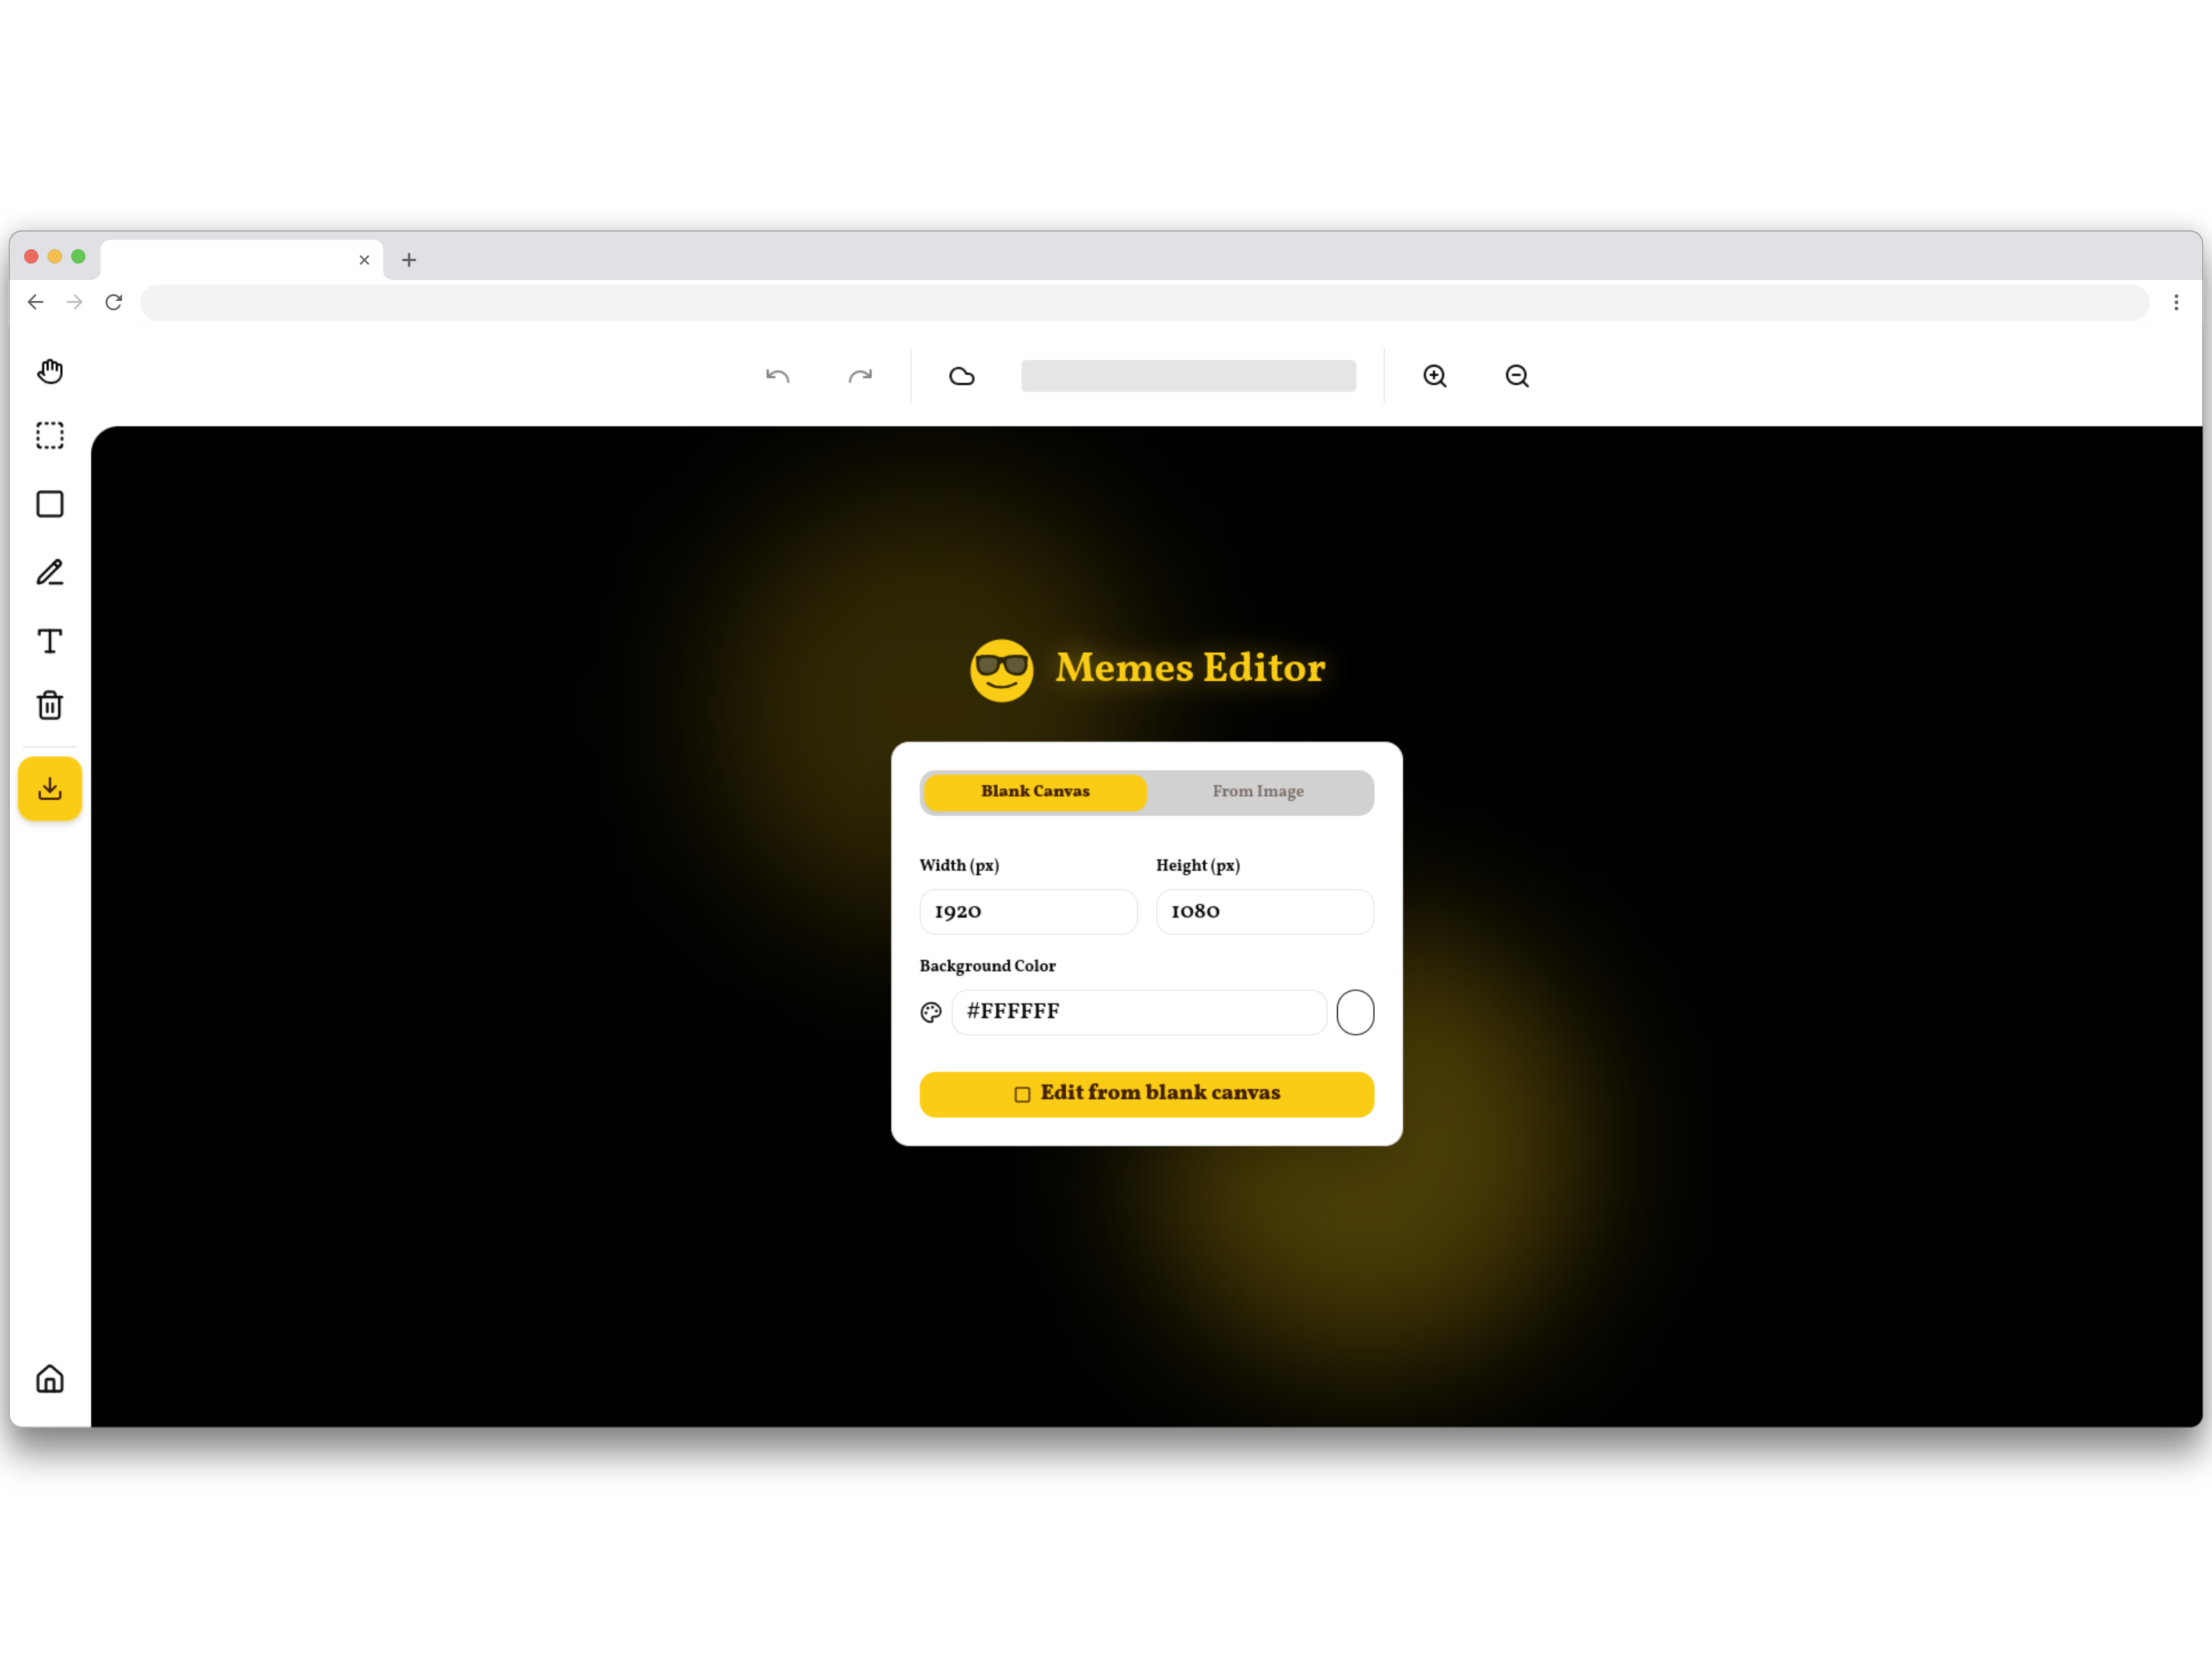
\includegraphics[scale=0.11]{figuras/editor_tema_claro.png}
\end{figure}

Para poner en contexto la explicación siguiente, se ha mostrado una captura actual del editor. En la parte izquierda se encuentran las diferentes herramientas para interactuar con el canvas, en la parte superior se encuentran las opciones más referentes al almacenamiento y gestión de estado y en la parte central se encuentra el componente principal, el canvas.

\subsubsection{Componente principal: Canvas}

El componente principal del editor es el canvas, cuya gestión completa está a cargo de Fabric.js, ya explicada anteriormente y que proporciona, de forma nativa, herramientas robustas para gestionar figuras, interacciones y personalizaciones dentro del canvas, lo que lo convierte en una elección ideal para este tipo de proyectos.

\subsubsection{Inicialización del canvas}

Siguiendo las mejores prácticas de Fabric.js para entornos React, se utiliza el hook useEffect para controlar la inicialización del canvas. Este enfoque garantiza que:

\begin{itemize}
    \item La instancia del canvas se cree antes de que el componente sea renderizado, asegurando que esté completamente disponible para su manipulación.
    \item Exista una única instancia del canvas durante el ciclo de vida del componente, evitando así la creación innecesaria de múltiples instancias.
    \item Cuando el componente se desmonta, se realiza una limpieza adecuada del canvas para liberar recursos y evitar problemas de memoria o rendimiento.
\end{itemize}

\subsubsection{Enfoque orientado a objetos de Fabric.js}

Fabric.js adopta un enfoque claro de programación orientada a objetos (POO), lo que lo hace altamente intuitivo para desarrolladores familiarizados con este paradigma. La creación de la instancia del canvas sigue un patrón estándar en POO:

\begin{itemize}
    \item Se genera un objeto del canvas mediante la palabra clave \texttt{new}.
    \item Se pasan las opciones de configuración iniciales como argumentos, lo que permite personalizar el comportamiento y las propiedades del canvas desde el momento de su creación.
\end{itemize}

\subsubsection{Gestión de objetos en el canvas}

Uno de los aspectos más poderosos de Fabric.js es su enfoque modular y orientado a objetos para la gestión de los elementos dentro del canvas. Cada figura u objeto gráfico se trata como una entidad independiente, que puede añadirse, modificarse o eliminarse del canvas sin afectar a los demás elementos. Esto ofrece una gran flexibilidad, permitiendo:

\begin{itemize}
    \item Manipulación granular de cada objeto dentro del canvas.
    \item Edición y personalización independiente de cada elemento gráfico, mejorando la modularidad del código.
\end{itemize}

Este diseño modular fue un factor clave en la elección de Fabric.js para el proyecto, ya que facilita la construcción de aplicaciones complejas donde cada componente gráfico necesita ser tratado de manera autónoma y flexible.

\subsubsection{Inicialización nuevo proyecto}

Como se ha visto en la captura de pantalla del editor anteriormente insertada, en el componente principal no aparece como podemos ver en otros editores el lienzo en blanco, sino que, por el contrario, aparece un formulario con una serie de opciones para la creación personalizada de este lienzo. Se puede configurar tanto si partir desde un lienzo vacío o desde una imagen que el usuario importe. Cualquiera de las dos opciones crea un canvas de manera responsiva, es decir, adaptándose al ancho de la pantalla disponible manteniendo la relación de aspecto de la imagen original (por lo que una vez el meme resultante se exporte, tendrá las dimensiones inicialmente configuradas).

Si seleccionamos la opción de empezar el nuevo proyecto desde un lienzo vacío, se pueden configurar las dimensiones del lienzo y el color de fondo.

De lo contrario, si se selecciona la opción de empezar desde una imagen, se puede importar una imagen desde el dispositivo y empezar con nuestro meme a partir de ella.

\begin{figure}[H]
    \caption{Formulario nuevo proyecto desde imagen tema oscuro.}
    \centering
    \vspace*{0.5cm}
    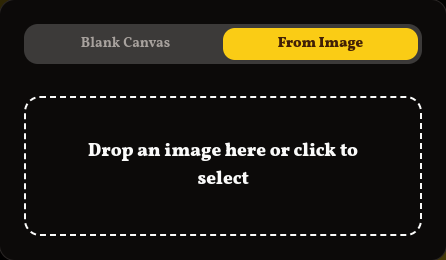
\includegraphics[scale=0.5]{figuras/meme_imagen_oscuro.png}
\end{figure}

Una vez se haya cargado el lienzo con nuestra configuración seleccionada se puede empezar a trabajar sobre el mismo.

\subsubsection{Inserción de imágenes}

Otro de los objetos para añadir al canvas es la imagen. Para ello, se ha implementado un sistema de carga de imágenes desde el dispositivo. Si queremos añadir cualquier imagen al canvas, se puede hacer desde la barra izquierda que más adelante mencionaremos o arrastrando la imagen directamente al canvas. Al hacer esto, se desenfoca el canvas, dando retroalimentación al usuario de que suelte la imagen para insertarla en el canvas.

\subsubsection{Barra izquierda: Herramientas}~\label{subsec:barra_izquierda}

\begin{figure}[H]
    \caption{Barra de herramientas en móvil y escritorio.}
    \centering
    \vspace*{0.5cm}
    \includegraphics[scale=0.2]{figuras/barra_movil_escritorio.png}
\end{figure}

En la barra izquierda se encuentran básicamente las herramientas que se pueden utilizar para la gestión de objetos del canvas. Estas herramientas son (de arriba a abajo):

\begin{itemize}
    \item \textbf{Arrastre}: permite hacer un barrido de cámara usando gestos táctiles (más pensado para móvil).
    \item \textbf{Selección}: permite seleccionar un objeto para poder moverlo, redimensionarlo, rotarlo, etc.
    \item \textbf{Rectángulo}: permite añadir un rectángulo.
    \item \textbf{Dibujo}: permite habilitar el modo dibujo para poder realizar trazos.
    \item \textbf{Texto}: permite añadir un texto.
    \item \textbf{Limpiar todo}: aplica una limpieza total, eliminando todos los objetos e historial para deshacer y rehacer.
    \item \textbf{Añadir imagen}: permite añadir una imagen.
\end{itemize}

Por último, tenemos la opción de guardar meme representada con un botón amarillo con un icono de descarga. Al hacer clic en este botón, se abrirá un modal o un cajón (si el dispositivo es móvil) en el que podremos seleccionar si guardarlo como imagen en el dispositivo o guardarlo en un catálogo de memes. Esta implementación se explicará más adelante en la sección de la integración con la capa de persistencia de datos.

Aparte, existe el icono de una casa que nos lleva a la página principal de la aplicación.

\subsection{Barra superior: Operaciones}

\begin{figure}[H]
    \caption{Barra superior de operaciones.}
    \centering
    \vspace*{0.5cm}
    \includegraphics[scale=0.2]{figuras/barra_operaciones.png}
\end{figure}

En la barra superior se encuentran las operaciones más referentes al almacenamiento y gestión de estado. Estas operaciones son (de izquierda a derecha):

\begin{itemize}
    \item \textbf{Deshacer}
    \item \textbf{Rehacer}
    \item \textbf{Guardar}: estado actual del meme. Si hacemos clic en este botón y estamos en un meme ya guardado se guardará el estado actual del mismo. De igual manera, cada minuto se guarda automáticamente. Sin embargo, si estamos en un meme nuevo, se notificará al usuario para que guarde el meme en un catálogo. De forma pasiva, este botón informa de cuando hay cambios sin guardar con un círculo amarillo pulsante.
    \item \textbf{Nombre de meme}: indica el nombre del meme actualmente.
    \item \textbf{Aumentar zum}
    \item \textbf{Disminuir zum}
\end{itemize}

\subsubsection{Propiedades de las figuras}

Esta sección es independiente a las demás debido a que dependiendo del dispositivo del usuario se mostrarán las propiedades en la barra superior o en la inferior (si el dispositivo es móvil).

\begin{figure}[H]
    \caption{Propiedades de las figuras.}
    \centering
    \vspace*{0.5cm}
    \includegraphics[scale=0.2]{figuras/propiedades_objetos.png}
\end{figure}

Como se puede apreciar en la figura, las propiedades de las figuras se muestran de acuerdo a las establecidas manualmente en el momento o configuradas en el objeto seleccionado. En el caso del rectángulo las propiedades modificables son el color de relleno, del borde y la anchura del borde. En el caso del texto, las propiedades modificables son el color del texto, la tipografía y el estilo. Por último, en el caso del trazado las propiedades modificables son el color y la anchura.

\section{Milestone 4: Integración almacenamiento-editor}

Este milestone se centra en la integración del editor con la capa de persistencia de datos asegurando que los memes elaborados desde cero o modificados en el editor puedan ser almacenados y gestionados en el sistema. Finalmente, como parte de este hito, se desplegará la aplicación en un entorno de producción.

Esta integración engrasa las partes hasta ahora realizadas en el proyecto, permitiendo que la aplicación tenga un flujo completo de interacción con los memes.

Para empezar a explicar esta parte, se va a organizar por páginas o rutas de la aplicación.

\subsection{Página principal: Catálogos}

\begin{figure}[H]
    \caption{Página principal y listado de catálogos.}
    \centering
    \vspace*{0.5cm}
    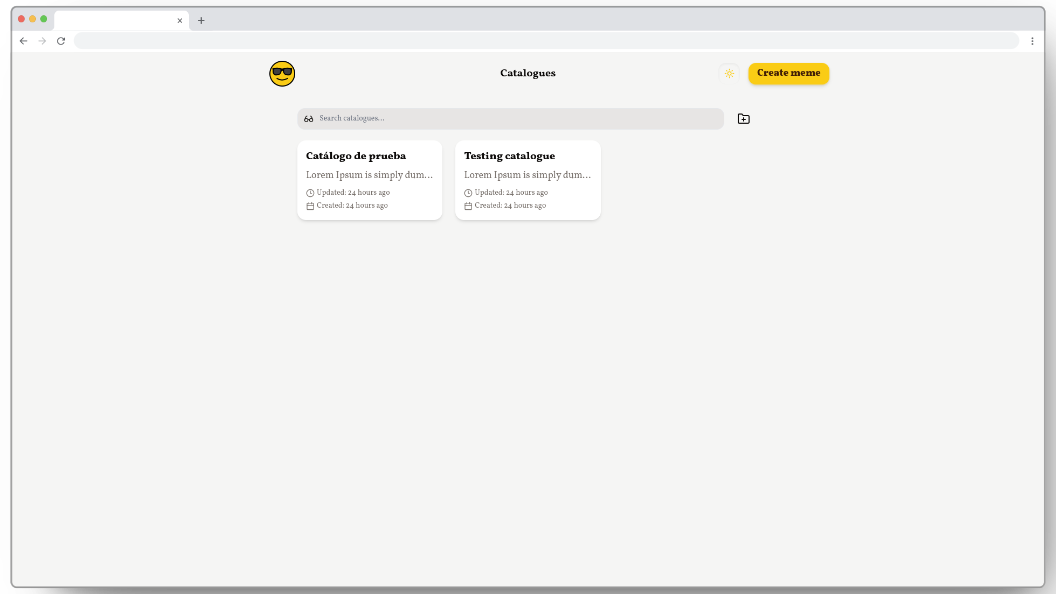
\includegraphics[scale=0.33]{figuras/catalogos.png}
\end{figure}

Cuando se accede a la página principal de la aplicación se muestra la lista de catálogos que actualmente existen en la base de datos. Cuando se pasa el ratón por encima de un catálogo, se muestra un botón para poder eliminarlo y si se hace clic, se redirige a la página de memes que contiene el mismo.

Cabe destacar que antes de eliminar un catálogo, se muestra un modal de confirmación para evitar la eliminación accidental junto con un conteo de los memes que contiene el catálogo (si los contiene).

\begin{figure}[H]
    \caption{Botón del catálogo.}
    \centering
    \vspace*{0.5cm}
    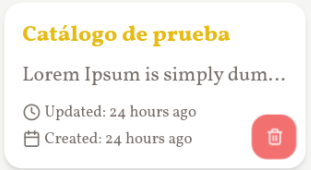
\includegraphics[scale=0.4]{figuras/card_catalogo.png}
\end{figure}

Ya tenemos la parte de eliminación y acceso por parte del catálogo, pero, ¿cómo se crea un catálogo? Para ello, se ha implementado un botón flotante en la parte derecha del buscador el cual se explicará más tarde. Una vez se haga clic en este botón, se abrirá un modal con un formulario. En este formulario se puede introducir el nombre del catálogo y una descripción opcional. Al enviar el formulario, se generará el catálogo y se cerrará el modal.

\begin{figure}[H]
    \caption{Formulario de creación de catálogo.}
    \centering
    \vspace*{0.5cm}
    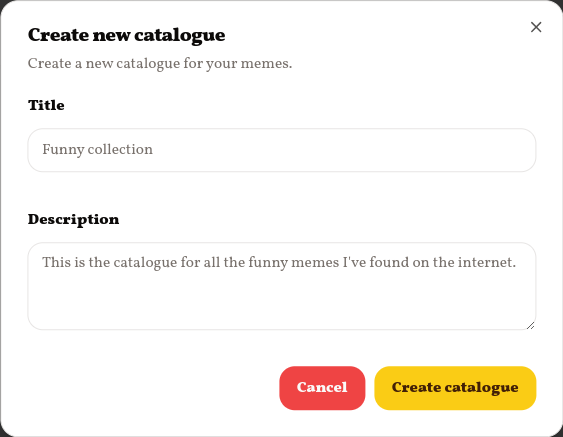
\includegraphics[scale=0.3]{figuras/card_creacion_catalogo.png}
\end{figure}

En nuestra aplicación, la forma de mostrar los catálogos es mediante una tarjeta que contiene el nombre, la descripción, la fecha de creación y actualización. El diseño de muestra de catálogos es de cuadrícula infinita responsiva, es decir, se adapta al ancho de la pantalla disponible.

A mayores, como se ha mencionado anteriormente existe una barra para realizar búsqueda de catálogos. Esta barra hace peticiones a la base de datos en tiempo real, es decir, a medida que se va escribiendo se van mostrando los catálogos que coinciden con la búsqueda. Esto funciona gracias a los \href{https://developer.mozilla.org/en-US/docs/Web/API/URL/searchParams}{searchParams} introducidos en la URL mientras el usuario escribe en la entrada de texto. Esta característica es muy útil para mejorar la experiencia de usuario, facilitar la búsqueda de catálogos y viene de la \href{https://developer.mozilla.org/en-US/docs/Web/API}{Web API}.

Una vez se selecciona un catálogo, se redirige a la página de memes que contiene el mismo.

\subsection{Página de catálogo: Memes}

\begin{figure}[H]
    \caption{Página de memes y listado de memes de un catálogo (modo oscuro).}
    \centering
    \vspace*{0.5cm}
    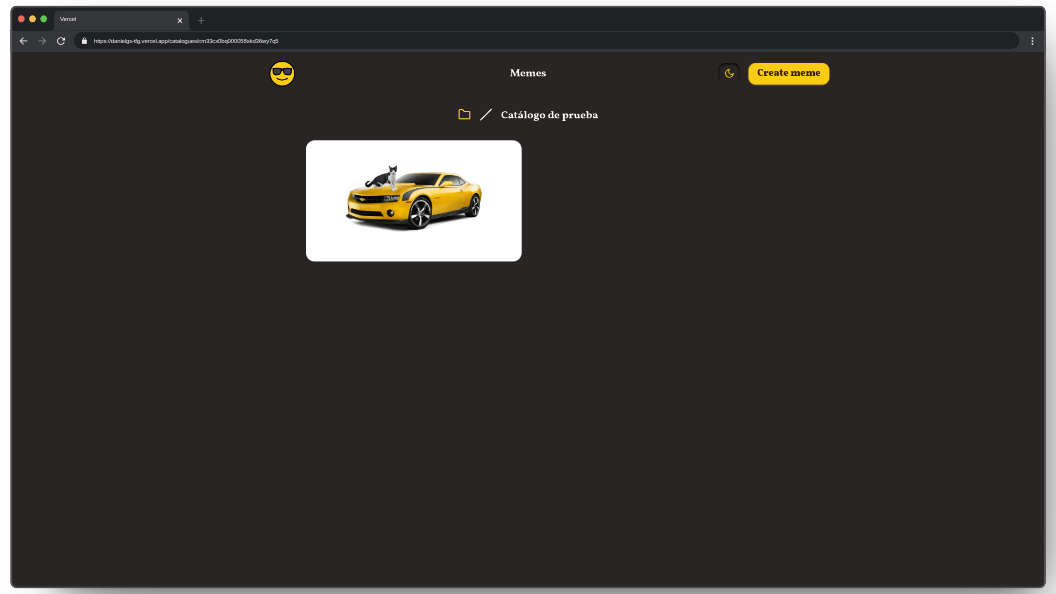
\includegraphics[scale=0.3]{figuras/memes.png}
\end{figure}

En la página de memes se muestra la lista de memes que actualmente existen en el catálogo. Al igual que en la página de catálogos, cuando se pasa el ratón por encima de un meme, se muestra un botón para poder eliminarlo, el nombre del meme, la fecha de modificación y creación y un botón para poder editarlo.

% textidote: ignore begin
Como se puede visualizar, la barra de direcciones la ruta ha cambiado por \texttt{/catalogo/\{id\}} donde el \texttt{\{id\}} es el identificador del catálogo seleccionado. Esta ruta dinámica se ha implementado gracias a la \href{https://nextjs.org/docs/app/building-your-application/routing/dynamic-routes}{API de rutas dinámicas del App Router de Next.js}. Esta API de rutas dinámicas permite crear rutas a partir de datos dinámicos y es muy útil para la creación de rutas personalizadas en nuestro caso, para algo tan cambiante como son los identificadores de los catálogos.
% textidote: ignore end

\begin{figure}[H]
    \caption{Tarjeta de un meme.}
    \centering
    \vspace*{0.5cm}
    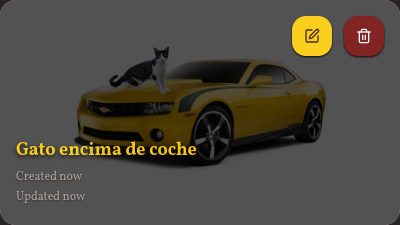
\includegraphics[scale=0.3]{figuras/meme_gato.png}
\end{figure}

Una vez se haga clic en el botón de editar, se redirige al usuario a la página del editor, pero con el meme seleccionado cargado en el canvas listo para ser editado.

\begin{figure}[H]
    \caption{Meme seleccionado en el editor.}
    \centering
    \vspace*{0.5cm}
    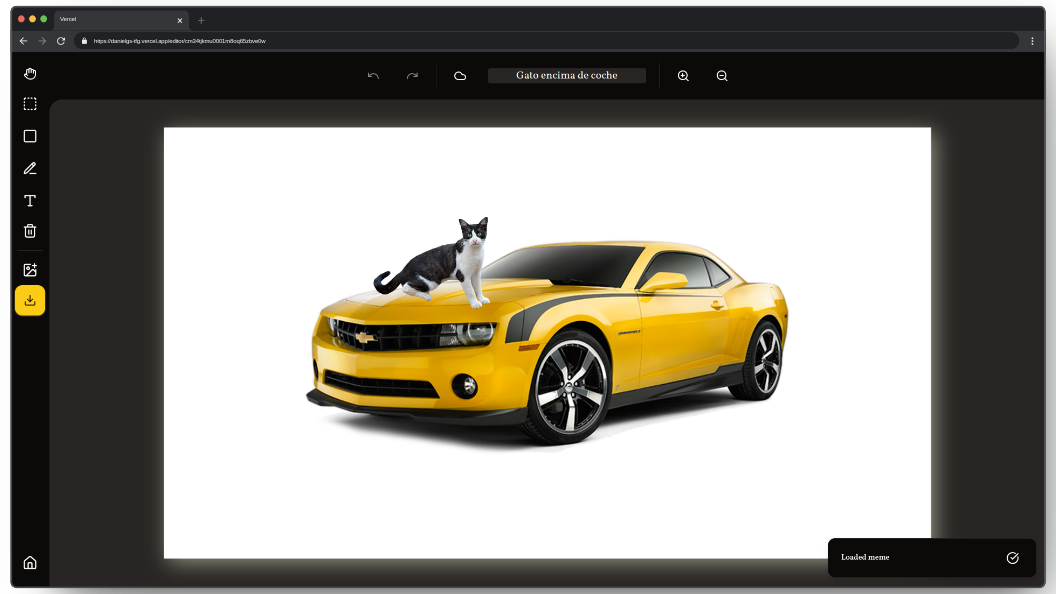
\includegraphics[scale=0.3]{figuras/meme_gato_editor.png}
\end{figure}

% textidote: ignore begin
Como se puede ver en la figura, el meme seleccionado anteriormente se ha cargado en el editor y se puede empezar a trabajar sobre él. En la barra de direcciones se puede ver que la ruta ha cambiado por \texttt{/editor/\{id\}} donde el \texttt{\{id\}} es el identificador del meme seleccionado. Como se ha mencionado anteriormente, esta ruta dinámica se ha implementado gracias a la API de rutas dinámicas del App Router de Next.js.
% textidote: ignore end

Una vez se ha cargado el meme, una notificación aparecerá en la parte inferior derecha de la pantalla informando de que el meme se ha cargado correctamente. Esta notificación se ha implementado de forma casi nativa gracias al componente \href{https://ui.shadcn.com/docs/components/toast}{toast} de la librería de componentes ShadCN~\ref{subsec:shadcn} que se ha mencionado anteriormente.

Tras hacer la modificación deseada al meme cargado, se puede guardar el nuevo estado del meme haciendo clic al botón de la nube en la barra superior. Al hacer clic en este botón, se guardará el estado actual del meme y se notificará al usuario de que se ha guardado correctamente. Cada vez que se haga una modificación no guardada del meme, este botón mostrará un círculo amarillo pulsante. Cabe destacar que cada minuto se guarda automáticamente para evitar posibles pérdidas de datos mejorando la experiencia de usuario.

\begin{figure}[H]
    \caption{Diálogo y cajón para guardar meme (escritorio y móvil).}
    \centering
    \vspace*{0.5cm}
    \includegraphics[scale=0.2]{figuras/guardar_meme.png}
\end{figure}

Por último vamos a explicar el flujo del botón amarillo de guardar meme. Partimos de la explicación dada en~\ref{subsec:barra_izquierda} donde se mencionaba que al hacer clic en este botón se abriría un modal o cajón. En este modal o cajón se puede seleccionar si guardar el meme en local o en un catálogo. Si se selecciona la opción de guardarlo en local, se descargará el meme que actualmente esté en el editor con el nombre y extensión especificados en el formulario. Por otro lado, si se selecciona la opción de guardarlo en el catálogo, se guardará el meme en el catálogo seleccionado. Si no se selecciona ningún catálogo, se guardará en el catálogo por defecto.

\section{Tests}

En esta sección se va a proceder a explicar la parte del TDD o Test-Driven Development. Esto consiste en escribir los tests antes de escribir el código de la aplicación. De esta forma, se asegura que el código cumple con los requisitos y se evitan errores en el futuro.

\subsection{Tests unitarios}

Para ejecutar las pruebas unitarias anteriormente explicadas y como, efectivamente se ha decidido anteriormente, se ha utilizado Cypress~\ref{subsec:cypress}. El flujo de trabajo tanto en estos tests como con los sucesivos se ha realizado de igual manera. Primero, elaborando y pasando los tests en local y luego en el flujo de trabajo remoto de GitHub Actions.

Por cada una de las entidades de la aplicación se han elaborado tests unitarios para comprobar que las operaciones CRUD funcionan correctamente desde la implementación en TypeScript nativo. Estos tests como se ha mencionado anteriormente, cada vez que se hace un \texttt{push} a la rama principal, se ejecutan en el flujo de trabajo de GitHub Actions revisando que la funcionalidad de la aplicación sigue siendo correcta incluso con la adición de nuevas características.

\subsection{Tests de end to end}

Como se ha explicado anteriormente, estos se ocupan de verificar que la aplicación funciona correctamente de cara al usuario final y que las diferentes partes de la aplicación interactúan estén bien engrasadas, siendo los mismos de gran utilidad y donde se va a poner el foco.

Los tests end to end cubren toda la funcionalidad de la aplicación, desde la creación de un catálogo hasta la edición de un meme. En adición al marco de desarrollo de Cypress se ha incorporado un plugin para la realización de comprobaciones visuales debido a que la parte del editor de memes es muy visual y se necesita de este plugin para asegurar que el lienzo muestre lo que se espera.

Para aportar detalle a la explicación, vamos a ver un caso de ejemplo en el que un test falla y se interrumpe el despliegue~\ref{sec:despliegue}.

\begin{figure}[H]
    \caption{Diagrama de flujo de la integración continua.}
    \centering
    \vspace*{0.5cm}
    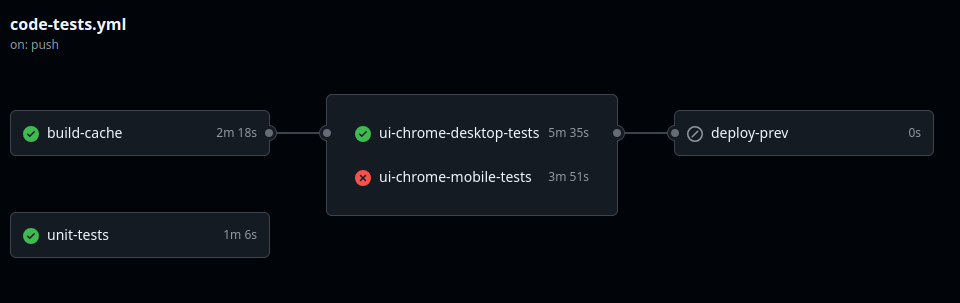
\includegraphics[scale=0.35]{figuras/fallo_test_e2e.png}
\end{figure}

Como se puede ver en la figura, el despliegue se ha interrumpido debido a que uno de los tests ha fallado. En este caso, uno relacionado con la versión móvil de la aplicación. Esto previene que se desplieguen versiones con errores y se asegura una calidad en el producto final.

Además de una interrupción en el flujo, Cypress como resultado genera un resumen para ver, a grandes rasgos, lo bien (o mal) que han ido.

\begin{figure}[H]
    \caption{Resumen de los tests de Cypress.}
    \centering
    \vspace*{0.5cm}
    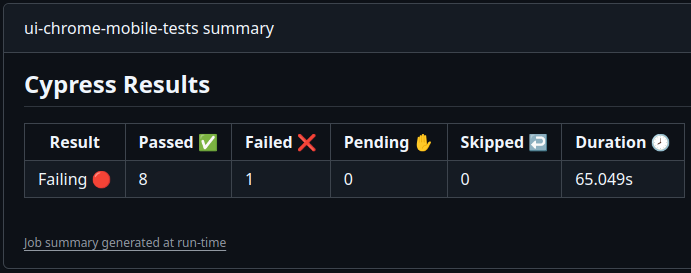
\includegraphics[scale=0.4]{figuras/resumen_cypress_ci.png}
\end{figure}

Una vez se haya identificado cuál ha fallado y por qué, se puede proceder a corregirlo lo cual puede ser trabajoso si no se tiene de un apoyo visual sobre qué se estaba probando. Para ello, se ha implementado una característica tanto en la configuración de Cypress como en la subida de artefactos de GitHub actions. Por la primera parte, se ha configurado que cada vez que falle un test, se tome una captura de pantalla del momento en el que ha fallado y por la otra parte que si esta carpeta existe y han fallado los tests que se suban las capturas realizadas.

\begin{figure}[H]
    \caption{Sección de artefactos de un workflow de GitHub Actions.}
    \centering
    \vspace*{0.5cm}
    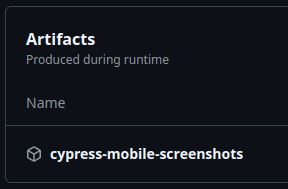
\includegraphics[scale=0.4]{figuras/artefacto.png}
\end{figure}

Como podemos ver, se suben en formato comprimido y se pueden descargar para visualizar en local y arreglar el error.

\begin{figure}[H]
    \caption{Captura de pantalla del test fallido.}
    \centering
    \vspace*{0.5cm}
    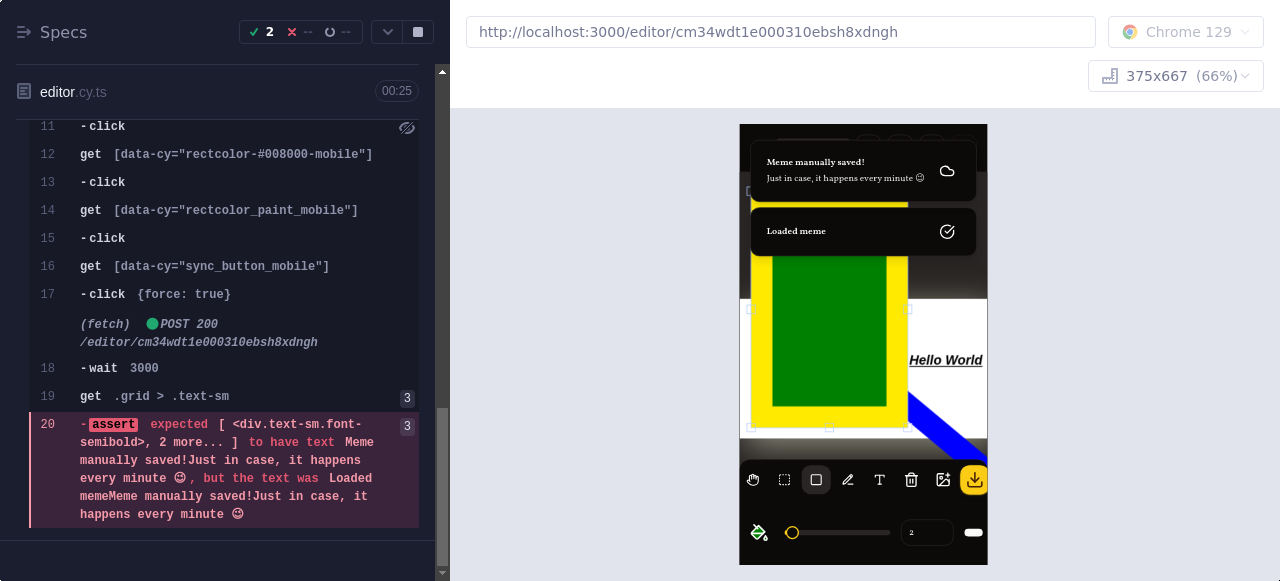
\includegraphics[scale=0.25]{figuras/test_fallado_snapshot.png}
\end{figure}

Como podemos ver, la captura de pantalla fue tomado justo en el momento en el que se detectó un error en las pruebas. Esto facilita la identificación del problema y su corrección, mejorando la eficiencia y la calidad del desarrollo.

\section{Despliegue}~\label{sec:despliegue}

El despliegue es el proceso mediante el cual se pone en funcionamiento una aplicación o sistema en un entorno accesible para los usuarios finales. En este caso, el despliegue implica transferir la aplicación desde el entorno de desarrollo (donde se desarrolla el código y las pruebas) a un servidor o plataforma en la nube, como Vercel, desde donde los usuarios podrán acceder a la aplicación de memes a través de internet.

El objetivo del despliegue es asegurar que el software esté disponible y funcione correctamente en el entorno real, permitiendo que los usuarios interactúen con él. En este proyecto, el despliegue se lleva a cabo en una plataforma en la nube que automatiza varios pasos del proceso, permitiendo actualizaciones y mejoras continuas sin interrumpir el servicio a los usuarios.  Esto permite entregar valor de forma constante y adaptarse a las necesidades cambiantes del usuario, asegurando que el sistema esté siempre actualizado y funcional~\cite{pressman2005software}.

En este proyecto, se ha optado por la plataforma de \href{https://vercel.com/home}{Vercel} debido a sus beneficios en términos de simplicidad, rapidez y escalabilidad. Esta es una plataforma de desarrollo web que permite a los desarrolladores no solo crear y desplegar aplicaciones web, sino también mantenerlas y escalar su rendimiento de manera sencilla. Entre sus principales características se destacan:

\begin{itemize}
    \item \textbf{Despliegue Continuo e Integrado}: Vercel facilita el proceso de integración y despliegue continuo (CI/CD), lo que permite implementar automáticamente las actualizaciones de código directamente desde el repositorio (GitHub, GitLab o Bitbucket), logrando así una experiencia de desarrollo fluida y colaborativa.
    \item \textbf{Optimización del Rendimiento}: Gracias a su infraestructura global, Vercel distribuye el contenido en múltiples regiones a través de una CDN, reduciendo la latencia y mejorando la velocidad de carga para los usuarios en diferentes ubicaciones.
    \item \textbf{Compatibilidad con Next.js}: Vercel es una plataforma optimizada para desplegar aplicaciones frontend, con integración destacada para frameworks como React, Vue.js y Svelte, pero especialmente con Next.js, desarrollado también por el equipo de Vercel. La reciente versión 15 de Next.js, lanzada el 21 de octubre, potencia aún más esta compatibilidad, permitiendo aprovechar sus ventajas sin complejidades adicionales. Con esta combinación, los desarrolladores pueden crear y desplegar aplicaciones de alto rendimiento, beneficiándose de funcionalidades avanzadas y un flujo de trabajo simplificado.
    \item \textbf{Experiencia de Usuario}: Vercel proporciona una interfaz amigable y herramientas analíticas avanzadas que permiten monitorizar el rendimiento y optimizar la aplicación en tiempo real.
\end{itemize}

Gracias a estas ventajas, Vercel representa una solución ideal para desarrollar, implementar y gestionar aplicaciones web modernas, asegurando rapidez, escalabilidad y una excelente experiencia tanto para los desarrolladores como para los usuarios finales.

Por último, cabe destacar que el plan \href{https://vercel.com/docs/accounts/plans/hobby}{Hobby de Vercel} (actualmente usado) es gratuito y permite desplegar aplicaciones de forma sencilla y sin coste adicional, lo que lo convierte en una opción atractiva para proyectos de desarrollo web de pequeña y mediana escala.

\subsection{Despliegue automatizado}

Como hemos podido ver anteriormente a modo de ejemplo en el flujo de trabajo de GitHub Actions de los tests, aparecía una última fase que era el despliegue. En esta fase se ha configurado una acción de GitHub que se encarga de desplegar la aplicación en Vercel automáticamente siempre y cuando los tests hayan terminado satisfactoriamente.

Estos despliegues automáticos se han dividido en dos entornos de despliegue: producción y preview.

En cada uno de los entornos de despliegue se ha configurado una serie de secretos de entorno para que la aplicación funcione correctamente en cada uno de ellos. Gracias a esta configuración se pueden desplegar las aplicaciones automáticamente y sin intervención manual, lo que mejora la eficiencia y la calidad del desarrollo. En la parte de GitHub existe una integración con el despliegue y estos entornos muy visual y accesible se puede ver el estado de los despliegues.

\begin{figure}[H]
    \caption{Despliegues en GitHub.}
    \centering
    \vspace*{0.5cm}
    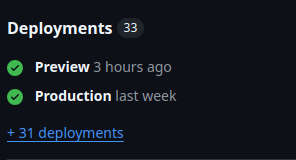
\includegraphics[scale=0.5]{figuras/despliegues.png}
\end{figure}

\subsubsection{Despliegue en producción}

El entorno de producción es el entorno final en el que se despliega la aplicación una vez se ha comprobado que todo funciona correctamente. Este entorno es el que se muestra a los usuarios finales y es el que se actualiza cada vez que se realiza un \texttt{push} a la rama principal.

En el caso de este entorno se ha configurado que solo se aplique a la rama principal, que se incorporen los secretos de entorno necesarios y que se despliegue en Vercel en producción.

\begin{figure}[H]
    \caption{Configuración de producción.}
    \centering
    \vspace*{0.5cm}
    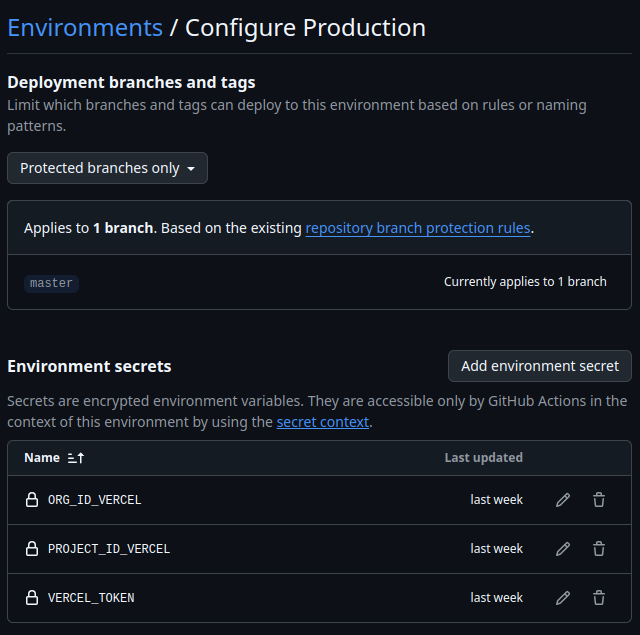
\includegraphics[scale=0.25]{figuras/entorno_prod.png}
\end{figure}

\begin{figure}[H]
    \caption{Producción.}
    \centering
    \vspace*{0.5cm}
    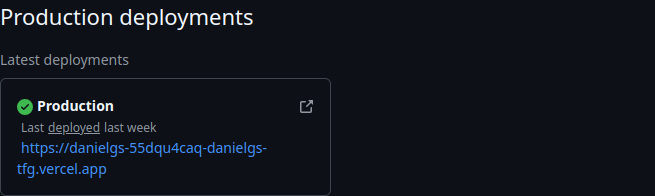
\includegraphics[scale=0.25]{figuras/despliegue_prod.png}
\end{figure}

\subsubsection{Despliegue en preview}

El entorno de preview es un entorno de despliegue temporal que se crea cada vez que se ejecuta un \texttt{pull request} a la rama principal. Este entorno es muy útil para probar que las nuevas funcionalidades o correcciones funcionan correctamente antes de ser desplegadas en producción.

Para el caso del entorno de preview se ha configurado para que se aplique a las ramas que no sean la principal y que contentan \texttt{m4/preview/*}, que se incorporen los secretos de entorno necesarios y que se despliegue en Vercel en preview.

\begin{figure}[H]
    \caption{Configuración de preview.}
    \centering
    \vspace*{0.5cm}
    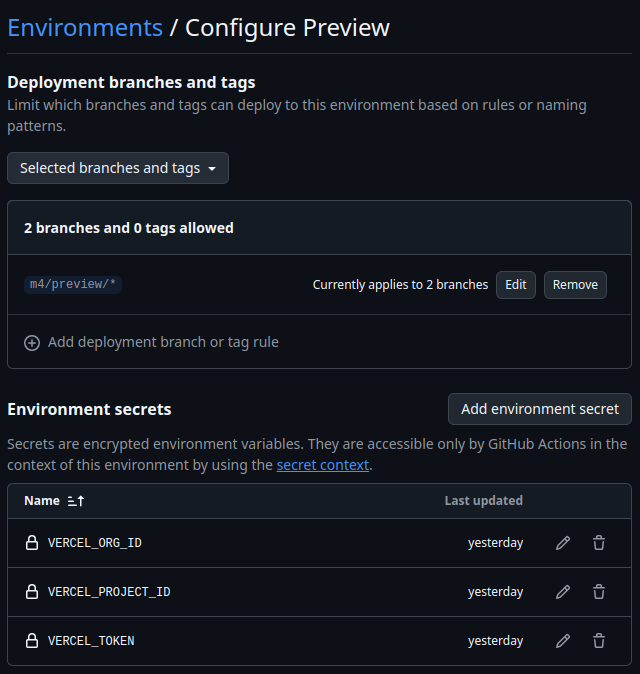
\includegraphics[scale=0.35]{figuras/entorno_prev.png}
\end{figure}

\begin{figure}[H]
    \caption{Preview.}
    \centering
    \vspace*{0.5cm}
    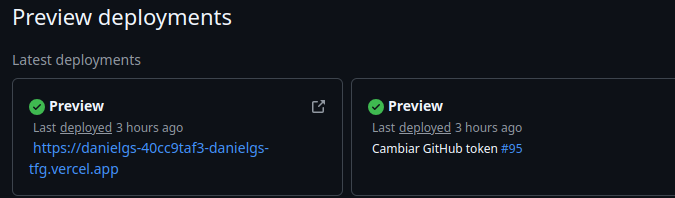
\includegraphics[scale=0.35]{figuras/despliegue_prev.png}
\end{figure}

\subsection{Despliegues en Vercel}

Una vez se ha desplegado la aplicación en Vercel en producción, se puede acceder a ella a través de la URL proporcionada por la plataforma. En este caso, la URL de la aplicación es \textbf{\href{https://danielgs-tfg.vercel.app/}{https://danielgs-tfg.vercel.app/}}.

En la página de nuestro proyecto en Vercel se pueden ver los despliegues, los entornos de despliegue y el estado de los mismos.

\begin{figure}[H]
    \caption{Página de despliegues en Vercel.}
    \centering
    \vspace*{0.5cm}
    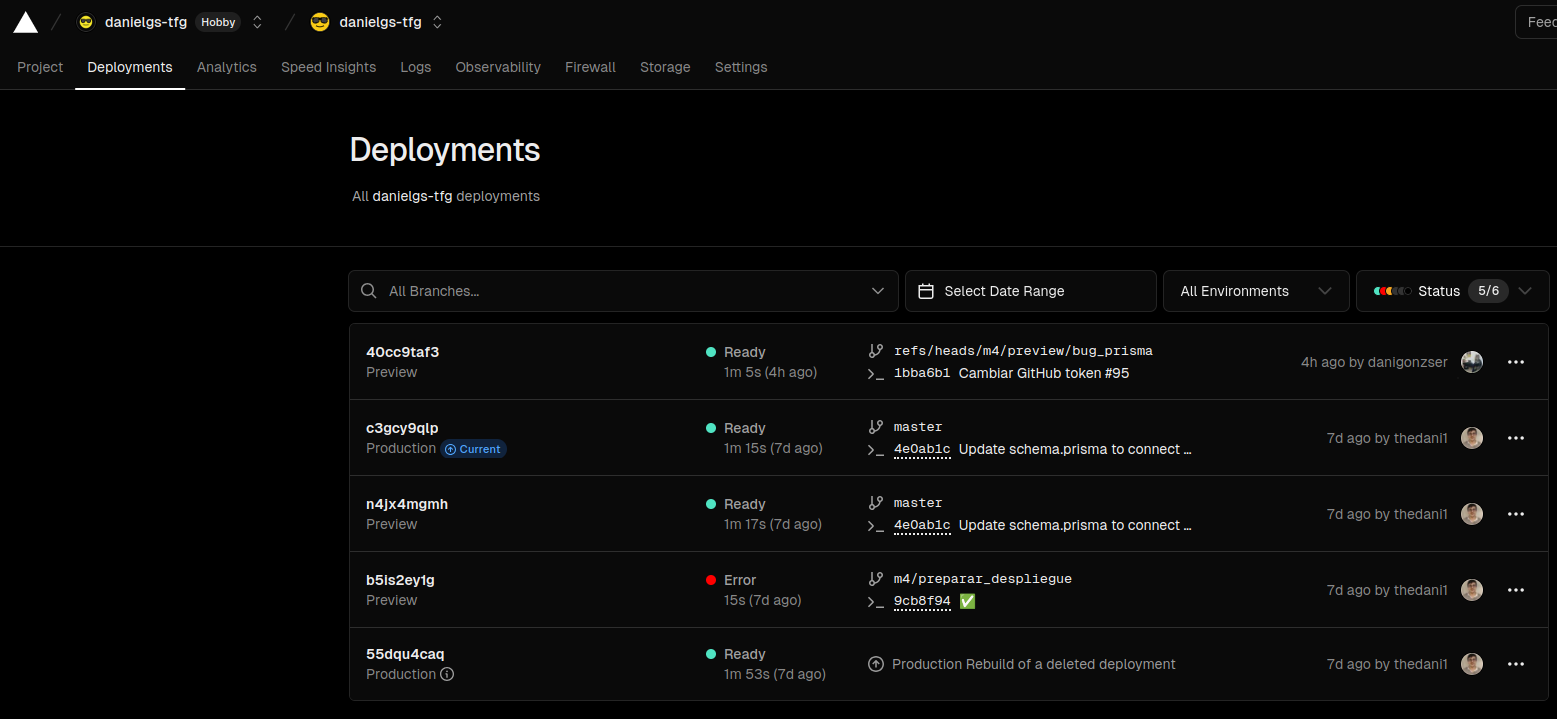
\includegraphics[scale=0.2]{figuras/despliegues_vercel.png}
\end{figure}

\subsubsection{Vercel Postgres}

En el caso de este proyecto, la capa de persistencia de datos se había utilizado Prisma y PostgreSQL por lo que en producción debía de ser igual. Para ello, se ha optado el servicio que ofrece el mismo Vercel.

\href{https://vercel.com/docs/storage/vercel-postgres}{Vercel Postgres} es una potente solución de base de datos en la nube diseñada para integrarse de forma nativa en la infraestructura serverless de Vercel, enfocada en aplicaciones web modernas que requieren escalabilidad y eficiencia. Al aprovechar la estructura sin servidor, Vercel Postgres permite a los desarrolladores escalar automáticamente sus bases de datos según la demanda, eliminando la necesidad de gestión manual de infraestructura y reduciendo costos operativos. Con una integración directa con Next.js y el ecosistema de Vercel, simplifica el flujo de desarrollo, permitiendo manejar bases de datos y aplicaciones en un mismo entorno, lo que facilita el despliegue y la configuración rápida. Además, su compatibilidad con la API estándar de PostgreSQL permite el uso de herramientas y bibliotecas populares sin esfuerzo adicional, lo cual, junto con su alto nivel de seguridad y la optimización para baja latencia, hace que sea una opción ideal para usuarios que buscan un rendimiento y una administración simplificados en sus proyectos web.